\documentclass[11pt]{article}
\usepackage[margin=1in]{geometry}
\usepackage{amsmath}
\usepackage{amssymb}
\usepackage{booktabs}
\usepackage{longtable}
\usepackage{array}
\usepackage{multirow}
\usepackage{xcolor}
\usepackage{caption}
\usepackage{graphicx}
\usepackage{subcaption}
\usepackage{float}
\usepackage{setspace}
\usepackage{natbib}
\bibliographystyle{agsm}
\usepackage{hyperref}
\hypersetup{colorlinks=true,linkcolor=blue,citecolor=blue,urlcolor=blue}

% [PL C0] PL suggested two titles. Applied her second option, which carries the
% governance argument. Her first was "Critical minerals and armed conflict:
% Evidence from Africa". Previous title was "Minerals, Markets, and Armed
% Conflict: Critical Minerals in the Modern Green Economy".
\title{Critical Minerals, Governance and Armed Conflict: \\ Evidence from Africa}
\author{Elisa D'Amico\thanks{University College Dublin. Email: elisa.damico@ucd.ie} \and P\"aivi Lujala\thanks{University of Oulu}}
\date{\today}

\begin{document}

\maketitle

% [PL C1] Cut to the 200-word journal limit. Recount after the results settle.
\begin{abstract}
\noindent The clean energy transition has sharply increased global demand for critical minerals. Yet many critical minerals are concentrated in regions with weak governance and histories of resource-related conflict. Africa, which holds substantial reserves of many critical minerals, sits at the center of this emerging challenge. Despite the strategic importance of these resources, systematic evidence on how critical mineral extraction shapes conflict dynamics remains limited. We analyze mineral discovery and armed conflict across Africa (1995--2018) using staggered difference-in-differences at multiple spatial scales. Our findings indicate that governance structure, and not mineral type alone, shapes conflict outcomes. Discoveries of internationally governed minerals such as tantalum pacify surrounding areas, as do nationally governed platinum group metals. Minerals that fall outside such governance structures show a decoupling pattern of fewer conflicts but higher lethality when violence occurs. Actor-level decomposition reveals that international governance pacifies all actor types, national governance excludes formal armed groups, and governance gaps see formal groups disappear while state-initiated lethality and civilian casualties increase. These results suggest that extending governance frameworks to strategic minerals currently lacking oversight could prevent the emergence of new ``blood minerals'' as the energy transition accelerates.
\end{abstract}

\section{Introduction}

The global energy transition is reshaping Africa's strategic importance. The continent holds substantial reserves of minerals needed for batteries, semiconductors, and renewable energy infrastructure \citep{iea2021critical}. Yet the relationship between mineral wealth and conflict in Africa remains contested. The conflict literature on mineral resources shows that extractive industries can fuel violence through competition over rents, funding of armed groups, and weakening of state institutions \citep{ross2004does, collier2004greed, lujala2009deadly, lujala2010spoils, fearon2005primary}. More recent work suggests these dynamics may be conditional on governance structures, environmental factors, and the specific characteristics of different minerals \citep{bazzi2019promises, berman2017mine, sanchez2020mining, buhaug2015climate, vonuexkull2016civil, koubi2019climate}. We contribute to this literature by examining how critical minerals\footnote{Critical minerals are those designated by major economies as strategically important for technology and clean energy, and as vulnerable to supply disruption.} managed under different governance structures relate to armed conflict in Africa.

Critical mineral extraction in Africa operates under highly uneven governance structures, with some minerals regulated through international due diligence regimes, others governed by strong national legislation, and still others lacking formal oversight entirely. International initiatives such as Dodd-Frank Section 1502, the OECD Due Diligence Guidance for Responsible Supply Chains of Minerals from Conflict-Affected and High-Risk Areas, and the International Tin Supply Chain Initiative emerged in the early 2010s in response to evidence that armed groups in eastern Democratic Republic of Congo were financing violence through the illicit trade of tin, tantalum, tungsten, and gold (3TG). These frameworks did not ban these minerals. They introduced transparency, traceability, and responsible-sourcing requirements that pressured downstream companies to map supply chains and avoid conflict financing. National governance can also reshape mineral sectors, as illustrated by South Africa's 2002 Mineral and Petroleum Resources Development Act, which replaced a fragmented private mineral-rights regime with state custodianship, licensing, and social and environmental obligations. Yet many critical minerals, chromium among them, remain outside both international and national governance systems, leaving extraction largely unregulated.

These divergent governance structures imply that the consequences of critical mineral discovery for conflict dynamics can vary. To study the relationship between critical minerals and conflict in Africa, we use geocoded data on critical mineral discoveries from 1997 to 2018, combined with conflict event data, at multiple spatial resolutions. We estimate the effect of mineral discovery on both conflict frequency and lethality. To study which actors are involved in the violence that follows discovery, we decompose conflict outcomes by the organizational type of the actors recorded in the UCDP Actor Dataset.

% [PL C40, C46] Mineral set fixed to tantalum / PGMs / chromium, and each mineral
% now introduced with its uses, African geography, and governance tier.
We focus on three critical minerals, each subject to a different form of governance.

Tantalum is one of the 3T minerals, alongside tin and tungsten, that fall under international due diligence frameworks. It is used almost entirely in capacitors for consumer electronics and in superalloys for aerospace and turbine components, and it has no close substitute at the performance levels these applications require. African tantalum is concentrated in the Great Lakes Region, above all in the eastern DRC and Rwanda, where much of it is mined artisanally from alluvial and pegmatite deposits by small, mobile workforces. That combination of high value per unit weight, low capital requirements, and dispersed workings is what made tantalum financeable for armed groups in the first place, and what put it at the center of the Dodd-Frank and ITSCI regimes. Tantalum is also the 3T mineral with enough treated grid cells to support estimation at our main resolution. Tin appears in the appendix as supporting evidence, and tungsten is discovered in too few cells, and too late in the panel, to estimate.

Platinum group metals comprise platinum, palladium, rhodium, and their companions, used in catalytic converters, hydrogen fuel cells, and electrolysers, which places them directly in the clean energy transition. Their African production is overwhelmingly South African, drawn from the Bushveld Complex, and extraction requires deep-shaft industrial mining with capital and engineering demands that put it beyond the reach of informal operators. This is the setting the MPRDA governs, and it is why PGMs serve here as the case of strong national governance.

Chromium is processed into ferrochrome and from there into stainless steel, superalloys, and the corrosion-resistant components used across industrial and energy infrastructure. African reserves sit mainly in southern Africa, again with the Bushveld Complex dominant, and in Madagascar and Zimbabwe. Extraction is industrial and open-pit or shallow-shaft rather than artisanal. No equivalent to Dodd-Frank or ITSCI covers chromium, and it is not subject to a national regime comparable to the MPRDA in the countries where our discoveries fall, so it stands here as the governance-gap case.

% [PL C48] Revisit once the results section is final.
Our central finding is that governance structure appears to mediate the mineral-conflict relationship in systematic ways. We identify three distinct patterns based on the governance regime surrounding each critical mineral. Minerals subject to international governance frameworks show consistent reductions in both conflict events and deaths, and the actor-level decomposition shows this applies across actor types, with state forces, formal armed groups, and civilians all seeing reduced violence. Supply chain transparency requirements appear to pacify areas with 3T minerals, potentially by defunding armed groups through the disruption of their access to mineral revenues \citep{parker2016resource, stoop2018dodd, bloem2022conflict}.

Nationally governed minerals reduce conflict through state monopoly control, with effects concentrated among formal armed groups \citep{cawood2004mineral}. National governance excludes formal armed groups from the conflict landscape without altering state or civilian outcomes.

Strategic minerals lacking governance frameworks exhibit a troubling ``decoupling'' pattern. Conflict events do not fall, but battle deaths rise, so violence becomes deadlier when it occurs. Formal armed groups are absent, while state-initiated fatalities and civilian casualties increase, consistent with state forces asserting control over strategically valuable but institutionally unregulated deposits.

These findings have direct policy implications. As demand grows for minerals central to the energy transition, extending governance frameworks to currently ungoverned strategic minerals could prevent the emergence of new resource conflicts, or the exacerbation of existing ones.

% [PL C409 / ED C410] Placeholder. Both authors flagged this as needing substance.
Our paper contributes to the large literature on \ldots

% [PL C61] Check all cross-references once the section merge is settled.
The rest of the paper is structured as follows. Section \ref{sec:governance} provides a brief introduction to the different governance frameworks under which critical minerals are governed in Africa and states our hypotheses. Section \ref{sec:data} describes our data and methodology. Section \ref{sec:results} presents the results and discusses the study's limitations. Section \ref{sec:discussion} discusses the implications of our findings, and Section \ref{sec:conclusion} provides concluding remarks and directions for further research.

\section{Critical Minerals, Governance Structures and Armed Conflict}
\label{sec:governance}

% [PL C77] PL rewrote this section without track changes, so it is a fresh draft
% rather than an edit of the previous "Governance-Value Nexus" section.

Mining of critical minerals in Africa is governed under different frameworks. Some minerals fall under international due diligence,\footnote{Due diligence refers to the process by which companies identify, assess, and mitigate risks in their mineral supply chains, including risks of conflict financing and human rights abuse.} others are subject to strong national governance, while others still lack such frameworks altogether.

The international due diligence initiatives Dodd-Frank Section 1502, the OECD Due Diligence Guidance for Responsible Supply Chains of Minerals from Conflict-Affected and High-Risk Areas (OECD Due Diligence Guidance for Conflict Minerals hereafter), and the International Tin Supply Chain Initiative (ITSCI) emerged from different origins but converged on curtailing armed groups' access to conflict funding from mineral exploitation in the eastern Democratic Republic of Congo (DRC). In the early 2000s, civil society organizations and advocacy groups, the UN Security Council, and the UN Group of Experts highlighted illegal exploitation and trade in tin, tantalum, tungsten, and gold (3TG) by armed groups in the war-torn eastern DRC \citep{unsc2002panel, globalwitness2010gun, vogel2016terr}. This led to international pressure to ban mineral exports from the DRC and, more broadly, from the Great Lakes Region. The three initiatives established in the early 2010s did not seek to ban conflict minerals. Instead, they created pressure and guidance for responsible mineral sourcing through transparency and tracing, along the lines of the Kimberley Process for diamonds \citep{grant2012kimberley}.

In response to calls to curtail rebel access to conflict minerals, Dodd-Frank Section 1502 was enacted as part of the Dodd-Frank Wall Street Reform and Consumer Protection Act, passed by the US Congress and signed into law in 2010. Section 1502 includes a legal disclosure requirement for publicly listed US-regulated manufacturing companies that use 3TG minerals in their products. Such companies must investigate whether these minerals originated in the DRC or adjoining countries, assess whether their sourcing may have contributed to conflict, and disclose their findings annually \citep{whitney2015conflict}. The legislation aimed at curtailing the black market and its negative effects, including human rights abuses, in the DRC. Dodd-Frank Section 1502 functions primarily as a transparency mechanism, creating strong incentives for US-regulated manufacturing companies to avoid opaque supply chains and invest in responsible sourcing programs. Its disclosure requirement has pushed companies to map their supply chains, adopt the OECD Due Diligence Guidance for Conflict Minerals, and rely on upstream tracing schemes like ITSCI.

ITSCI is the International Tin Association's traceability and due diligence program for tin, tantalum, and tungsten (3T) minerals sourced from the Great Lakes Region. It started as a pilot in eastern DRC in 2010 and was formalized in 2011, the same year Dodd-Frank Section 1502 came into force. ITSCI operates at mine sites, trading points, and export hubs, tracking minerals from their origin and seeking to identify risks related to conflict financing or human rights abuses \citep{postma2021itsci}. In practice, ITSCI tags minerals at the mining site and traces their movement throughout the supply chain, recording these in a shared database and reporting system that companies use to demonstrate responsible sourcing. It also investigates incidents and trains local authorities. The program currently covers around 3,000 mines across Burundi, DRC, Rwanda, and Uganda \citep{itsci2026}.

The OECD Due Diligence Guidance for Conflict Minerals is a global standard for responsible mineral sourcing, providing a five-step due diligence framework. The first edition was published in 2011 and coincided with the passage of Dodd-Frank Section 1502, thereby providing companies with a practical method for compliance. Although the Guidance originally centered on 3TG supply chains in the Great Lakes Region, subsequent revisions have clarified that it applies to all minerals globally. The framework provides voluntary due diligence standards for companies sourcing minerals from conflict-affected and high-risk areas, defined broadly to include regions experiencing armed conflict, widespread violence, political repression, institutional weakness, insecurity, or human rights abuses \citep{cardona2024due}.

South Africa's Mineral and Petroleum Resources Development Act (MPRDA), enacted in 2002, is an example of a national mineral governance structure. It represents a fundamental restructuring of the country's mineral governance system. Prior to the MPRDA, South Africa's system allowed landowners or companies to hold private mineral rights outright. This had resulted in fragmentation, restricted government oversight, and entrenched inequalities rooted in colonial and apartheid-era property regimes. The MPRDA replaced this system by vesting all mineral rights in the state, establishing a licensing regime, and embedding environmental and social responsibility obligations to ensure a more accessible, regulated, and socially responsive extractive sector \citep{cawood2004mineral, cawood2004investment}.

Finally, some critical minerals in Africa fall outside international and national governance frameworks. No equivalent to Dodd-Frank or ITSCI exists for chromium mining and supply chains, so extraction occurs without the transparency requirements or conflict-free certification that govern 3T mining and trade. Critical minerals are therefore governed under very different structures across Africa. We exploit these differences and propose that the effect of critical mineral discovery on conflict depends on that structure. Figure \ref{fig:dag} summarizes our framework and hypotheses.

% [PL C78] Standing caveat: hypotheses and surrounding text may need revision once
% the results are final.

The international due diligence frameworks seek to disrupt revenue flows to armed groups, formalize extraction through certified supply chains, and raise the costs of violence by attaching reputational and legal risks to buyers. We thus expect that international governance will reduce both the frequency of conflict and its lethality by pacifying armed groups, thereby reducing civilian suffering.

\begin{quote}
\textbf{H1:} The discovery of critical minerals subject to international governance frameworks reduces the number of conflict events.
\end{quote}

\begin{quote}
\textbf{H2:} The discovery of critical minerals subject to international governance frameworks reduces battle-related deaths.
\end{quote}

We expect that national governance also reduces conflict, through state monopoly control and the limited opportunities for armed groups to contest state authority over extraction. Because national governance operates through domestic institutions rather than international supply chain pressure, pacification effects may be weaker or more geographically concentrated than under international frameworks. At the actor level, we expect formal armed groups to be specifically excluded, as state monopoly control targets organized challengers to extraction, reducing their activity both as initiators and as targets of violence.

\begin{quote}
\textbf{H3:} The discovery of critical minerals subject to strong national governance reduces conflict events.
\end{quote}

% [PL C79] PL asked whether to add a battle-deaths hypothesis for the national
% tier. We make no directional prediction here, for the reason given below.
% Flagged for her decision.
We do not state a corresponding prediction for battle deaths under national governance. State monopoly control gives a clear expectation about which actors are present, and therefore about the frequency of events, but no clear expectation about the lethality of the violence that remains.

% [PL C81] PL asked whether to simplify the governance-gap hypotheses. Note that
% H4 is not supported by our own chromium results, which show no clear decline in
% events. Options are to drop H4 and make this a lethality-only prediction, or to
% keep it and report it as unsupported. Currently kept and reported as unsupported.
% [PL C82] Rewrote the passage on why formal groups are absent. The previous
% version turned on a double negation that PL flagged as unreadable.
We expect critical minerals lacking a governance framework to exhibit a ``decoupling'' pattern, as the combination of high value and low oversight attracts state forces seeking to secure extraction sites. Formal armed groups have little foothold in this setting. Extraction of these minerals is industrial rather than artisanal, so it offers armed groups none of the dispersed, low-capital revenue opportunities that sustain them around 3T deposits, and there is no certification regime whose capture would be worth contesting. The expected result is fewer conflicts overall but deadlier ones, driven by state-initiated violence and civilian casualties.

\begin{quote}
\textbf{H4:} The discovery of critical minerals lacking governance frameworks reduces conflict events.
\end{quote}

\begin{quote}
\textbf{H5:} The discovery of critical minerals lacking governance frameworks increases battle deaths.
\end{quote}

\begin{figure}[H]
    \centering
    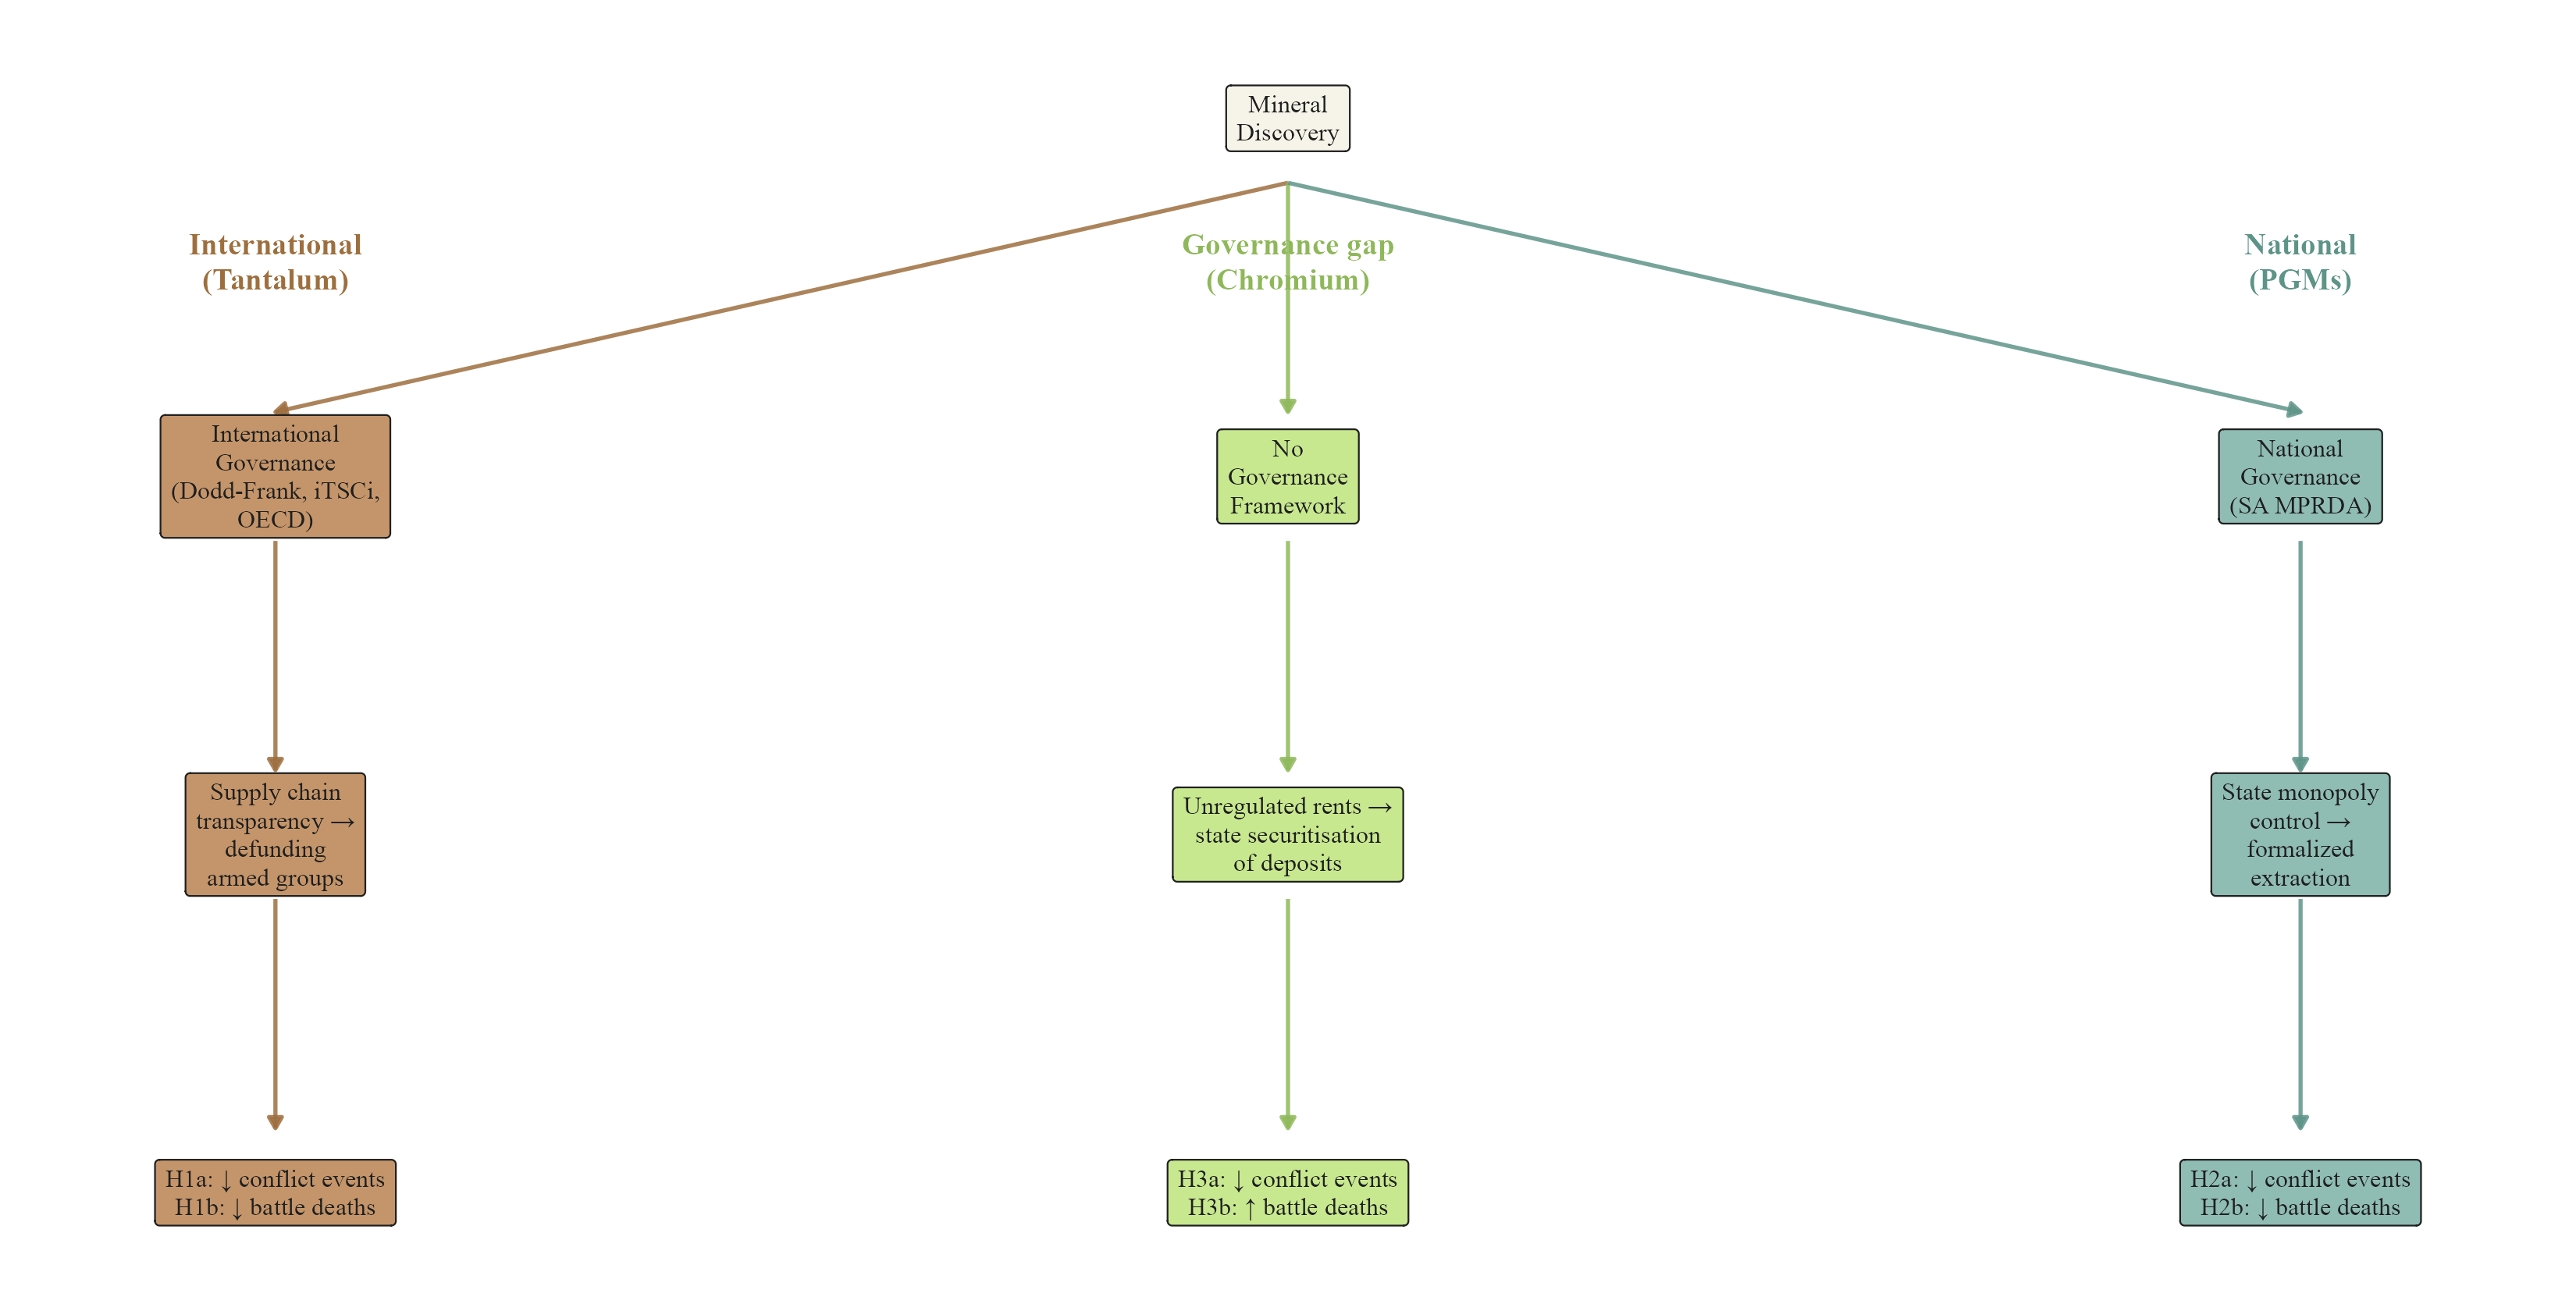
\includegraphics[width=0.85\textwidth, trim=150 50 150 70, clip]{plots/governance_value_dag.png}
    \caption{Theoretical pathways from mineral discovery to conflict outcomes. The effect of discovery depends on the governance regime, and each pathway produces distinct outcomes for conflict frequency and lethality.}
    \label{fig:dag}
\end{figure}

\section{Data and Methods}
\label{sec:data}

\subsection{Data}

Our dataset covers the years 1995--2018, with mineral discoveries recorded from 1997 onward, and we use hexagonal grid-year cells that cover the entire African continent as the unit of study. We construct hexagonal grid cells at seven spatial resolutions (25km to 300km diameter) to test robustness across scales. The main analysis uses 100km resolution, which balances local precision with sufficient conflict variation for estimation. Appendix Figure \ref{fig:africa_hex_grids} illustrates the grid structure at 50km and 300km resolutions, and Appendix Tables \ref{tab:tantalum_robustness}--\ref{tab:pgms_robustness} report results across all spatial scales.

% [PL C115] Descriptive figures computed from
% REM/data/hex_year_panel_100km_critical.rds.
At 100km resolution the continent is covered by 3,658 hexagonal cells, giving 87,792 cell-years. Discoveries are rare and spatially concentrated. Across all critical minerals in the database, 227 cells, or 6.2 percent of the total, record at least one discovery during the study period, spread over 316 cell-years. The three minerals analyzed here account for a small share of these. Tantalum is discovered in 25 cells, chromium in 11, and platinum group metals in 8. Tin, which we report in the appendix, is discovered in 12 cells. Tungsten reaches only 3 cells, with the first in 2013, which leaves too short a post-treatment window and too little variation for estimation, and it is therefore excluded.

Conflict is also sparse in the cells that receive discoveries, and unevenly so across the three tiers. Over the full panel the 25 tantalum cells record 335 conflict events and 12,664 battle deaths, with some conflict in 10.2 percent of their cell-years. The 8 PGM cells record 41 events and 286 deaths, with conflict in 6.2 percent of cell-years. The 11 chromium cells record 14 events and 35 deaths in total, with conflict in 2.7 percent of cell-years. Estimates for the nationally governed and governance-gap tiers therefore rest on a small number of treated cells and very few conflict events, and we return to what this implies for interpretation in Section \ref{sec:results}.

% [PL C115] Partly addressed. Still outstanding: the S&P inclusion criterion for
% an exploration record to count as a discovery, and the country distribution of
% discoveries. The latter needs a spatial join against national boundaries, which
% requires the sf package (not currently installed). The UCDP country field in the
% panel is populated only for cells that record conflict, so it cannot stand in.
To study the relation between critical minerals and violent conflict, we combine two data sources. First, mineral discovery locations come from the S\&P Global Market Intelligence database, which provides geocoded records of mineral exploration and discovery across Africa. We draw on 22 critical minerals recorded in the database, of which tantalum, platinum group metals, and chromium form the basis of the analysis reported here. Coverage runs to 2018, which sets the end of our study period.

% [PL C116] Rationale for discovery rather than production spelled out.
We focus on discoveries rather than production for two reasons. The first is timing. Discovery precedes extraction by years or decades, so it captures the point at which expectations about a location's mineral wealth change, before any of the roads, jobs, or revenue flows that accompany an operating mine can confound the comparison. The second concerns identification. Where a firm chooses to open a mine is not independent of local conditions, since companies avoid areas they judge too insecure to operate in, which means production onset is partly a consequence of the conflict environment we are trying to explain. The location of a mineral deposit, by contrast, is fixed by geology. What varies is when exploration happens to confirm it, and that timing is driven largely by world prices, exploration budgets, and survey technology rather than by conditions in the surrounding grid cell. Treating the confirmation year as the treatment date therefore comes closer to an as-if random assignment of when a place becomes known to be mineral-rich.

% [PL C119] Inclusion criteria, geocoding, and the battle-deaths definition added.
Second, conflict data come from the Uppsala Conflict Data Program Georeferenced Event Dataset (UCDP-GED v25.1) \citep{sundberg2013ucdp, pettersson2021organized}. UCDP-GED records individual instances of lethal organized violence, defined as the use of armed force between two organized parties resulting in at least one death. Events enter the dataset only if they belong to a conflict dyad that passes UCDP's annual threshold of 25 battle-related deaths, so isolated violence outside an active organized conflict is not captured. Each event carries a date and a geographic coordinate, together with a precision code recording how exactly the location is known, ranging from an exact site to a first-order administrative area or an entire country. We retain events geocoded at least to the level of a populated place or a second-order administrative unit, so that assignment to a grid cell is meaningful, and we assign each retained event to the hexagonal cell containing its coordinate.

From these data we code our primary dependent variables, namely (1) conflict event counts per grid cell, which capture overall conflict frequency, and (2) battle deaths per grid cell, which capture conflict intensity and lethality. Battle deaths are the fatalities UCDP attributes to a given event, counting combatants on both sides together with civilians killed in the course of the fighting. UCDP publishes low, best, and high estimates for each event, reflecting the range across the underlying source reports. We use the best estimate throughout, and we return in Section \ref{sec:results} to the uncertainty this introduces.

% [PL C135] Justified. The violence-type split is not used in the main results,
% which run on total event counts, but it does carry the spatial-scale robustness
% tables in Appendix A. Stated here so the reader knows where it appears.
We also record UCDP's classification of each event by type of violence, distinguishing state-based violence between a government and an armed opposition, non-state violence between two non-government actors, and one-sided violence against civilians. The main results use total event counts, since the three governance tiers differ in which types of violence occur at all near their deposits and a common outcome keeps them comparable. The disaggregation by violence type carries the spatial-scale robustness tables in Appendix \ref{sec:scales}, where it shows at which scales each tier's effect is concentrated in which kind of violence.

% [PL C143, C282] Actor definitions moved here from the mechanisms section, where
% PL flagged that "who is affected" was ambiguous.
To investigate the mechanisms behind our main results, we use the UCDP Actor Dataset (v25.1) to identify the organizational type of each conflict participant, distinguishing formal military organizations, political organizations, identity-based groups, state actors, and civilians. Every UCDP event records two sides, so each actor type enters our data in two distinct roles. An actor is an \textit{initiator} when it is the side that carried out the violence, and a \textit{target} when it is the side against which the violence was directed. We construct separate outcomes for each role, so that ``formal group initiator events'' counts events in which a formal armed organization used violence, while ``formal group target events'' counts events in which one was attacked. Each role is measured both as a count of events and as a count of battle deaths. This distinction matters for interpretation. A decline in formal group initiator fatalities means organized armed groups are killing less, whereas a decline in formal group target fatalities means fewer of their members are being killed, and the two need not move together.

% [PL C155, C163] DONE. Map rebuilt by REM/09_paper_figures.R with a white
% background, larger legend text, a distinct symbol per mineral, and raw rather
% than logged conflict counts. The old map (08_viz.R) classified gallium and
% germanium as the governance-gap tier, which predates the switch to chromium,
% so it was plotting minerals that are not in the analysis.
Figure \ref{fig:map} shows the distribution of conflict events and mineral governance tiers across Africa.

\begin{figure}[H]
    \centering
    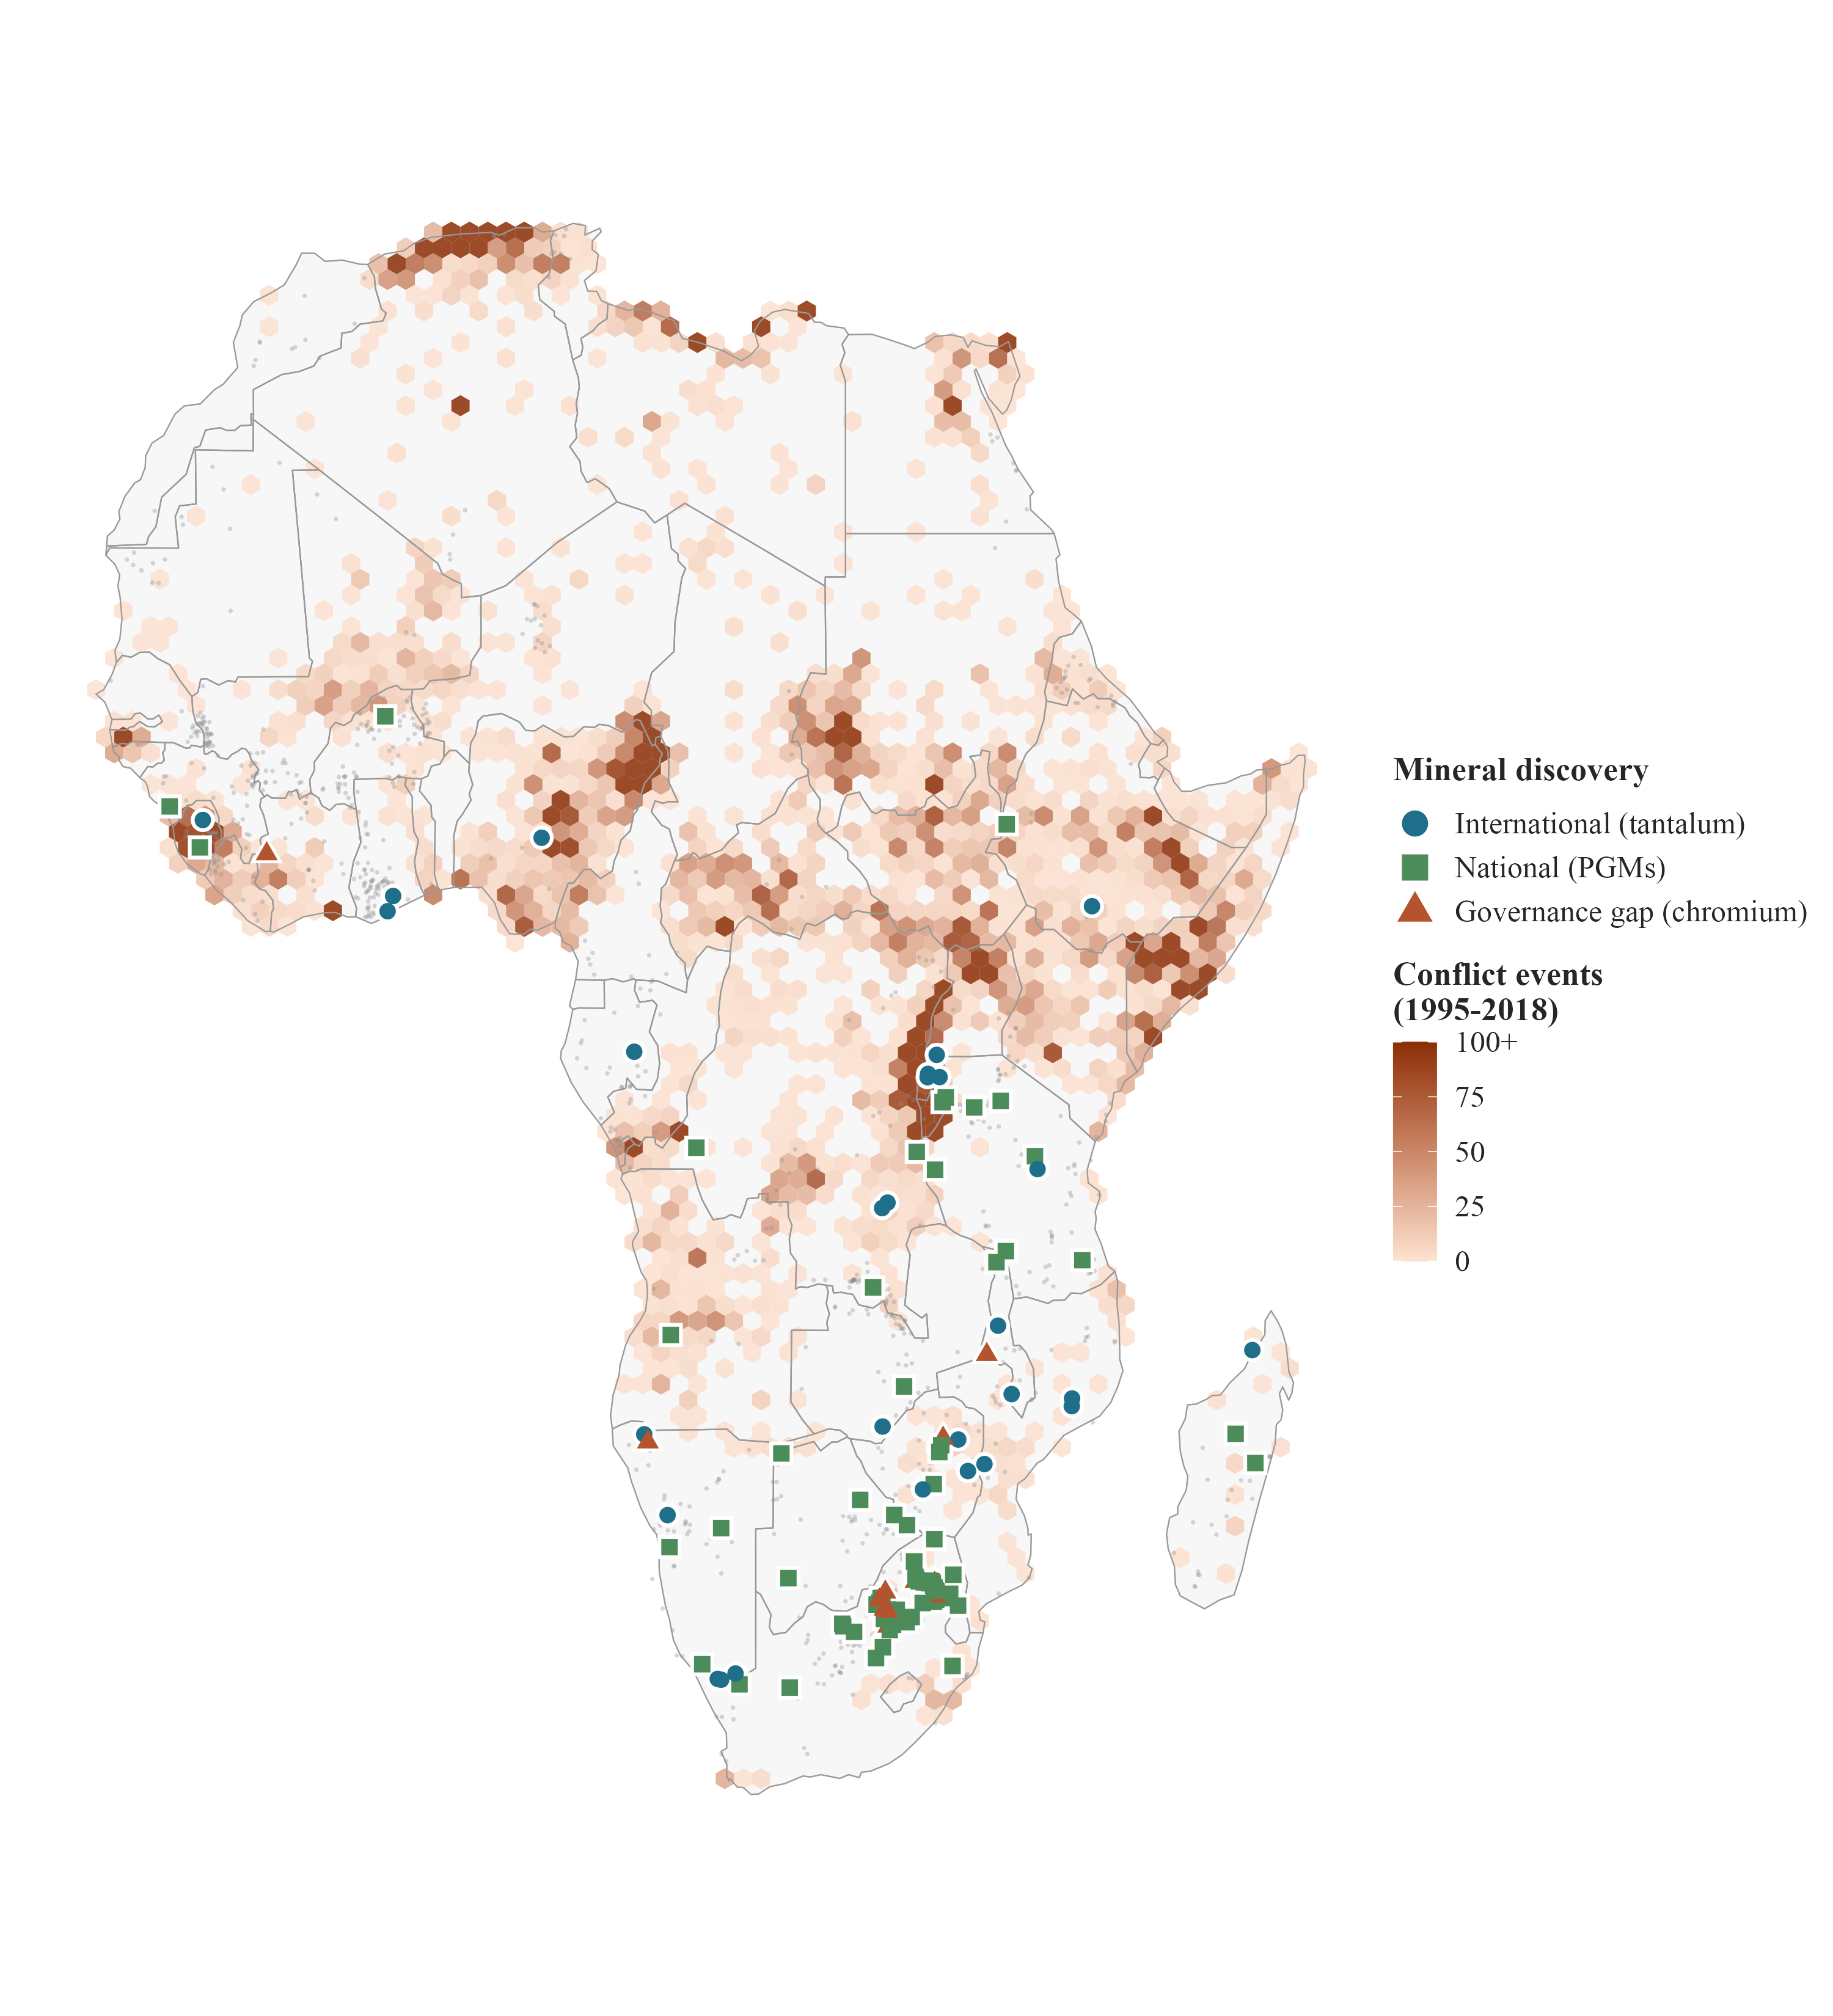
\includegraphics[width=0.65\textwidth]{plots/africa_mineral_conflict_map.png}
    \caption{Conflict events (1995--2018) and mineral discoveries across Africa, shown at 100km resolution. Hex cells are shaded by the raw count of conflict events, capped at 100 so the scale stays readable. Symbols mark discovery locations for the three analysed minerals, namely tantalum (international governance), platinum group metals (national governance), and chromium (governance gap). Small grey points mark discoveries of other critical minerals not analysed here.}
    \label{fig:map}
\end{figure}

\subsection{Empirical Strategy}

% [PL C167] PL drafted the plain-language explanation below. Still missing is the
% guidance on how to read the event-study figures (see the flagged sentence at the
% end of this subsection).
We estimate staggered difference-in-differences models using the approach of \citet{callaway2021difference}, which addresses bias from heterogeneous treatment timing \citep[see also][]{goodman2021difference, sun2021estimating}. Staggered difference-in-differences allows us to follow each grid cell over time and, if there is a mineral discovery in a given year, to compare that cell and its subsequent grid-years with cells that never experience a discovery anywhere in the panel.\footnote{The estimator can draw its comparison group either from cells not yet treated at a given point or from cells never treated at all. We use the never-treated pool throughout, which is the more conservative choice here because discovery cells are few and their treatment years are spread across the panel.} Put differently, staggered difference-in-differences compares what happens to different grid cells over time when they are treated at different moments, and uses those timing differences to estimate the treatment effect. The strength of this method is that it isolates the effect of mineral discovery on our conflict outcomes from other changes happening over time.

In our analysis, treatment is defined as the first mineral discovery in a grid cell. We estimate average treatment effects on the treated (ATT) for each post-treatment period. Our main specifications take the form

% [PL C217] Outcome notation generalized so it covers the actor-level outcomes as
% well as event counts and battle deaths.
\begin{equation}
Y_{it} = \alpha_i + \lambda_t + \sum_{k=-K}^{K} \beta_k \cdot \text{Discovery}_{it}^k + \varepsilon_{it}
\end{equation}

\noindent where $Y_{it}$ is the outcome in grid cell $i$ and year $t$, $\alpha_i$ are cell fixed effects, $\lambda_t$ are year fixed effects, and $\text{Discovery}_{it}^k$ is an indicator equal to one when cell $i$ is $k$ periods from first mineral discovery (with $k < 0$ for pre-treatment and $k \geq 0$ for post-treatment periods). In the aggregate analysis $Y_{it}$ is either the count of conflict events or the number of battle deaths. In the actor-level analysis it is the count of events or deaths for a given actor type in a given role, as defined above. The coefficients $\beta_k$ capture the dynamic treatment effects, with pre-treatment coefficients providing a test of parallel trends. We report results using the Callaway-Sant'Anna estimator, which aggregates group-time average treatment effects on the treated into event-study coefficients while accounting for heterogeneous treatment timing.

The identifying assumption for the impact of mineral discovery on our conflict outcomes is parallel trends. This means that prior to any grid cell being treated, all grid cells have roughly the same conflict trends over time up until the treated cell's discovery year. Put differently, if no grid cell had ever experienced a discovery, all grid cells would have continued to evolve in parallel. Any deviation after treatment is then attributed to the discovery rather than to other unrelated trends. We assess parallel trends by examining pre-treatment coefficients. Our specifications generally satisfy parallel trends, with most minerals showing zero to few significant pre-treatment periods.

% [PL C167] TO FINISH: explain how to read the event-study figures. PL's
% placeholder read: "In our figures, parallel trends show as a flat line... and
% treatment effect as departure from this line..."
Each event-study figure plots these coefficients against event time. Coefficients to the left of zero describe the years before discovery and should sit close to the horizontal line at zero if parallel trends hold. Coefficients to the right of zero describe the years after discovery, and a departure from the zero line there is the estimated treatment effect. Vertical bars give 95\% confidence intervals, so an interval that excludes zero indicates an effect distinguishable from no change.

% =====================================================================
% [PL C255] Sections 4 (Results), 5 (Mechanisms) and 6 (Production
% robustness) merged into a single Results section, with the study's
% limitations as the final subsection, per PL's proposal. Discussion is
% retained as its own section, since C255 named only sections 4-6.
% =====================================================================
\section{Results}
\label{sec:results}

\subsection{Aggregate Effects by Governance Tier}

% [PL C256] Placeholder minerals replaced with the final set.
We first present results for the three governance structure categories, namely internationally governed tantalum, nationally governed platinum group metals, and chromium, which is subject to neither international nor national governance. For each mineral we show results for conflict events and battle deaths at 100km resolution.

% [PL C257] DONE. The three separate paired event studies are replaced by one
% 3x2 figure, built by REM/09_paper_figures.R.
%
% !! WARNING - READ BEFORE EDITING THE RESULTS TEXT BELOW !!
% This figure is built from the CORRECTED panel (hex_year_panel_100km_critical_fixed.rds).
% The surrounding prose still describes the OLD estimates, which were computed on
% a treatment variable corrupted by the reduce()/left_join() bug documented in
% REM/10_fix_treatment.R. Figure and text therefore disagree. On the corrected
% data none of the six aggregate ATTs is significant. See REM/11_compare_fix.R
% for the side-by-side comparison. The results narrative needs rewriting before
% this section can be circulated.
Figure \ref{fig:main_results} presents event-study estimates for all three minerals, with conflict events in the left column and battle deaths in the right.

\begin{figure}[H]
    \centering
    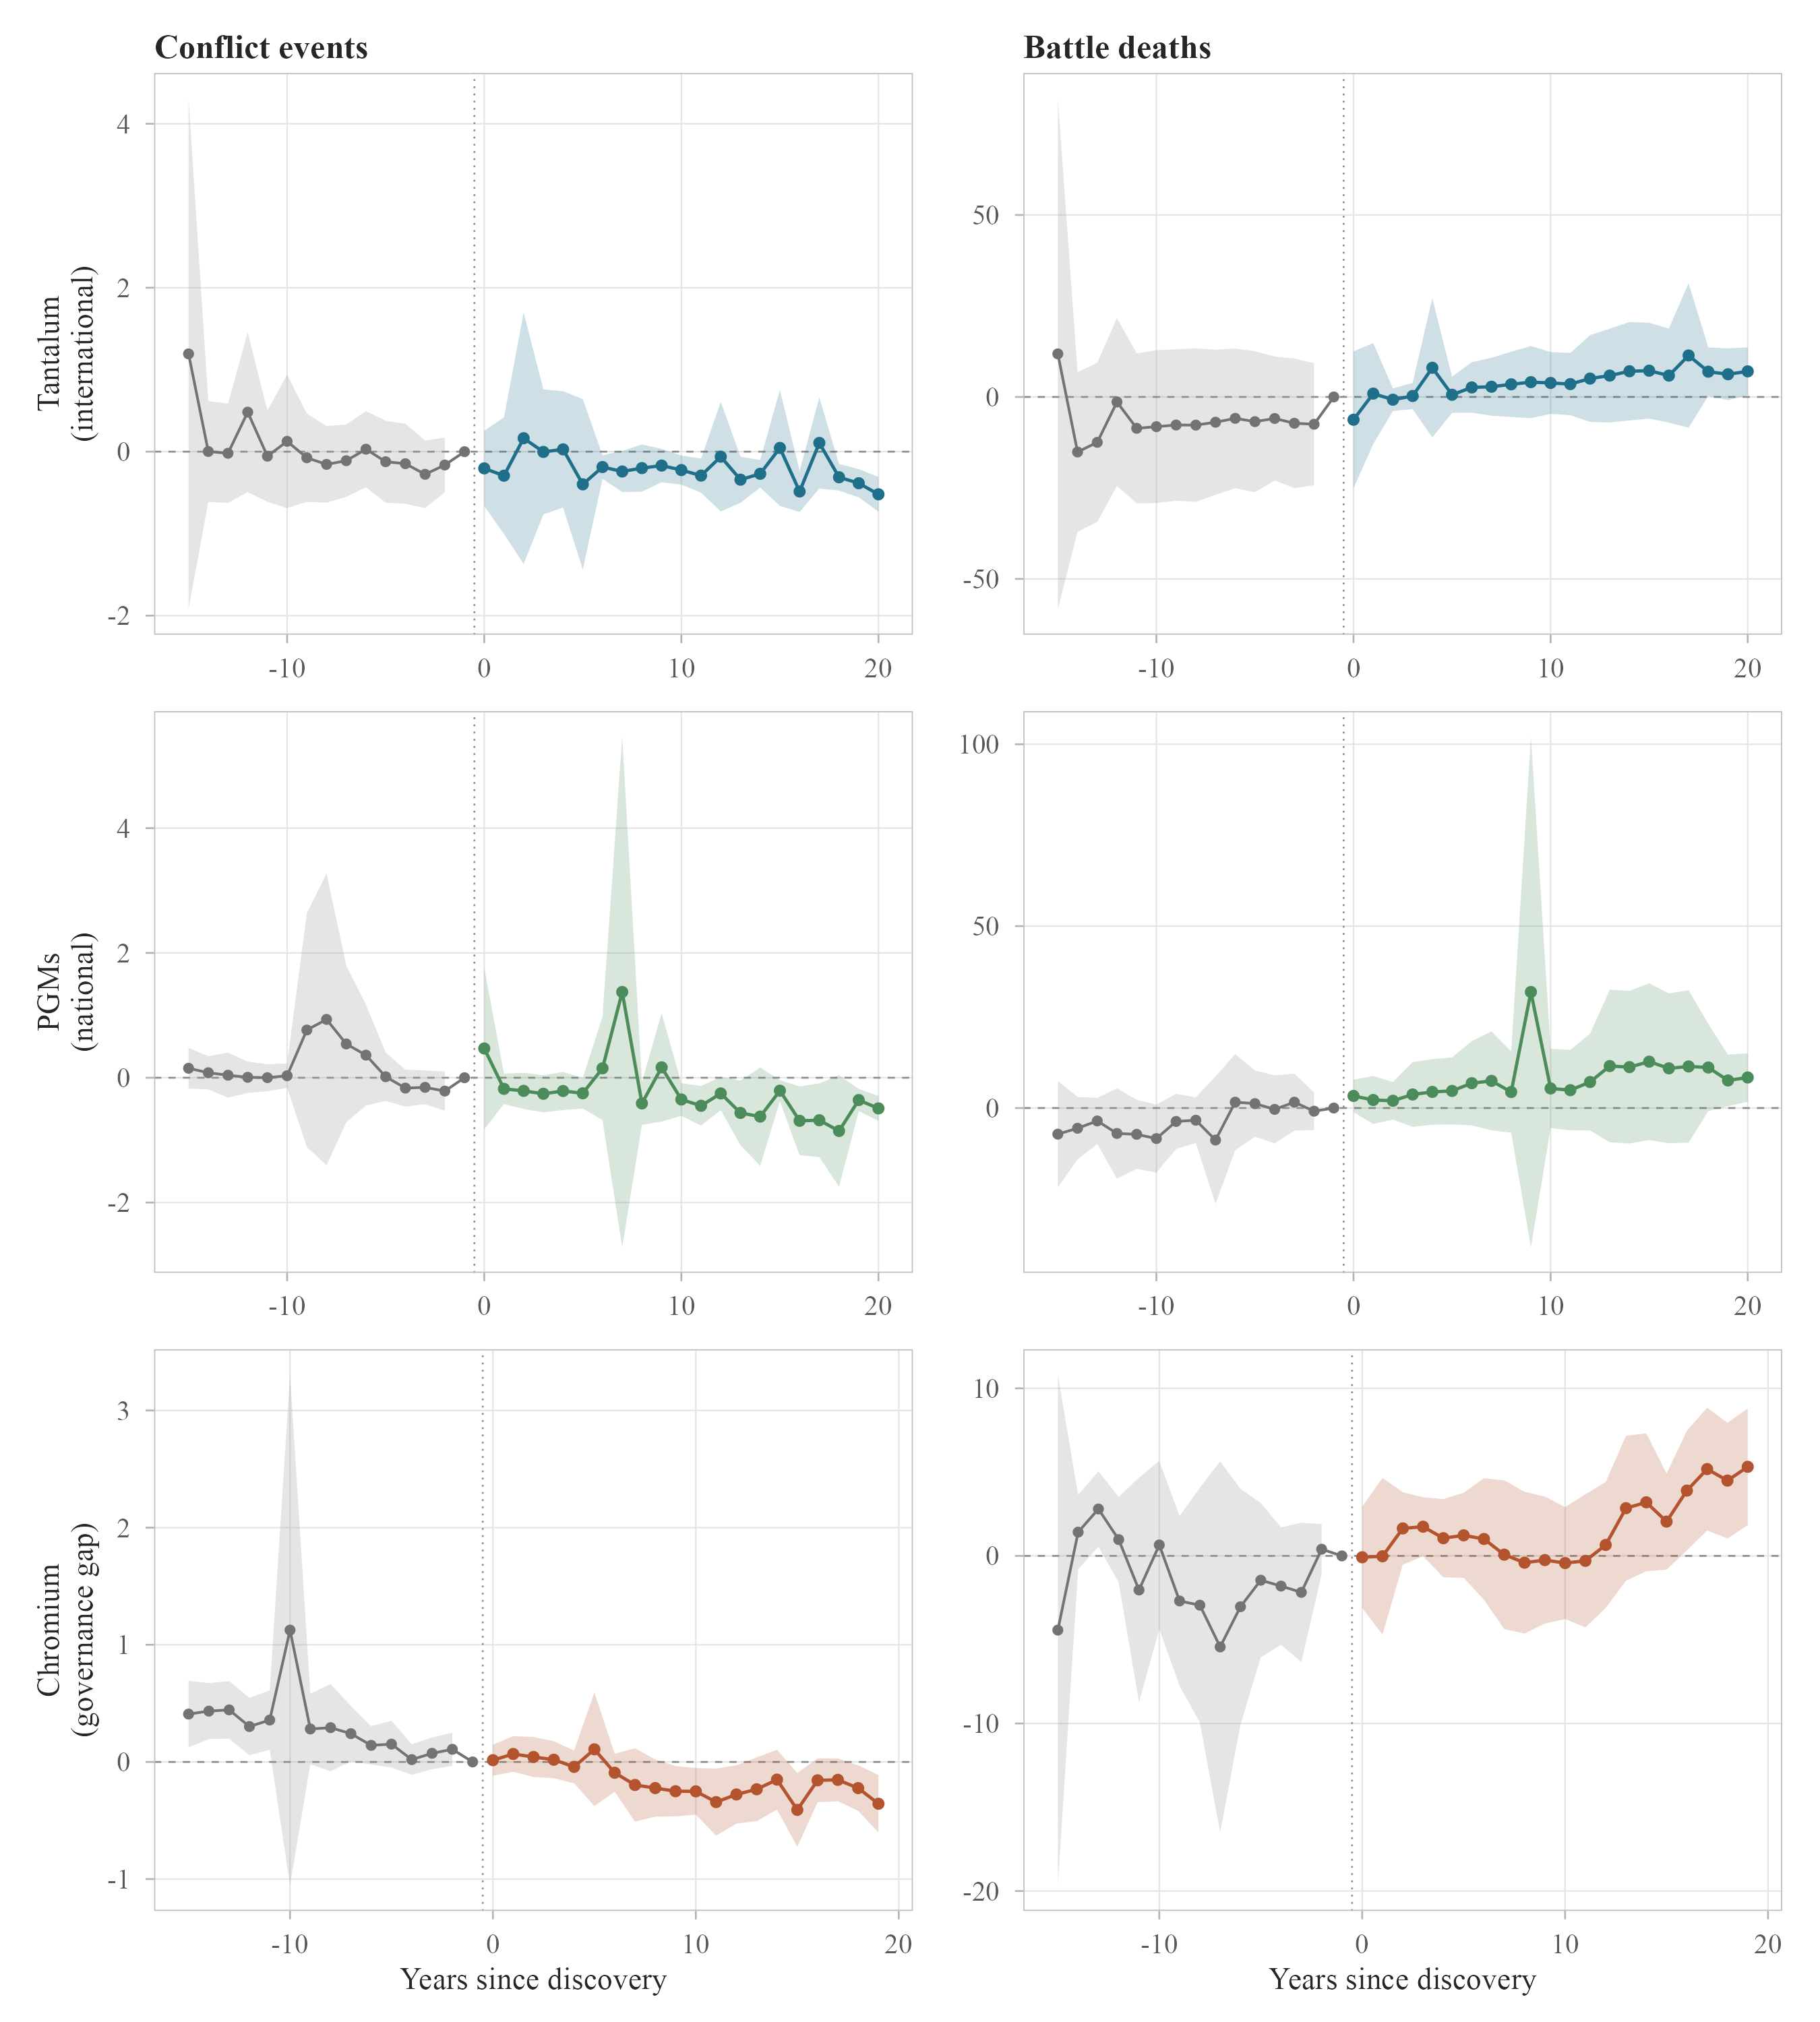
\includegraphics[width=0.92\textwidth]{plots/main_results_merged.png}
    \caption{Event-study estimates by governance tier at 100km resolution. Rows are tantalum (international governance, 25 treated cells), platinum group metals (national governance, 8 treated cells), and chromium (governance gap, 11 treated cells). The left column shows all conflict events, the right column battle deaths. Grey marks pre-treatment periods and colour marks post-treatment periods, with shaded bands giving 95\% confidence intervals. Estimates use the Callaway-Sant'Anna estimator with never-treated controls.}
    \label{fig:main_results}
\end{figure}

% [ED C277 / PL C278] Pooled-effects figure removed by agreement of both authors.
% The underlying table (latex/pooled_effects.tex) remains in Appendix C.

% [PL C279] PL could not read this figure and flagged the substantive issue that
% the governance interventions land in 2009-2011 while the panel opens in 1997.
% Connected to C39 (post-2010 subsample). Figure retained pending that decision.
Figure \ref{fig:calendar} presents the same patterns using a calendar-time specification aligned to policy milestones. Tantalum shows declining conflict after Dodd-Frank (2010) and the OECD guidelines (2011), consistent with governance frameworks driving pacification. Chromium shows battle deaths increasing without clear policy triggers, consistent with the absence of governance frameworks. PGMs show gradual decline beginning after South Africa's MPRDA.

\begin{figure}[H]
    \centering
    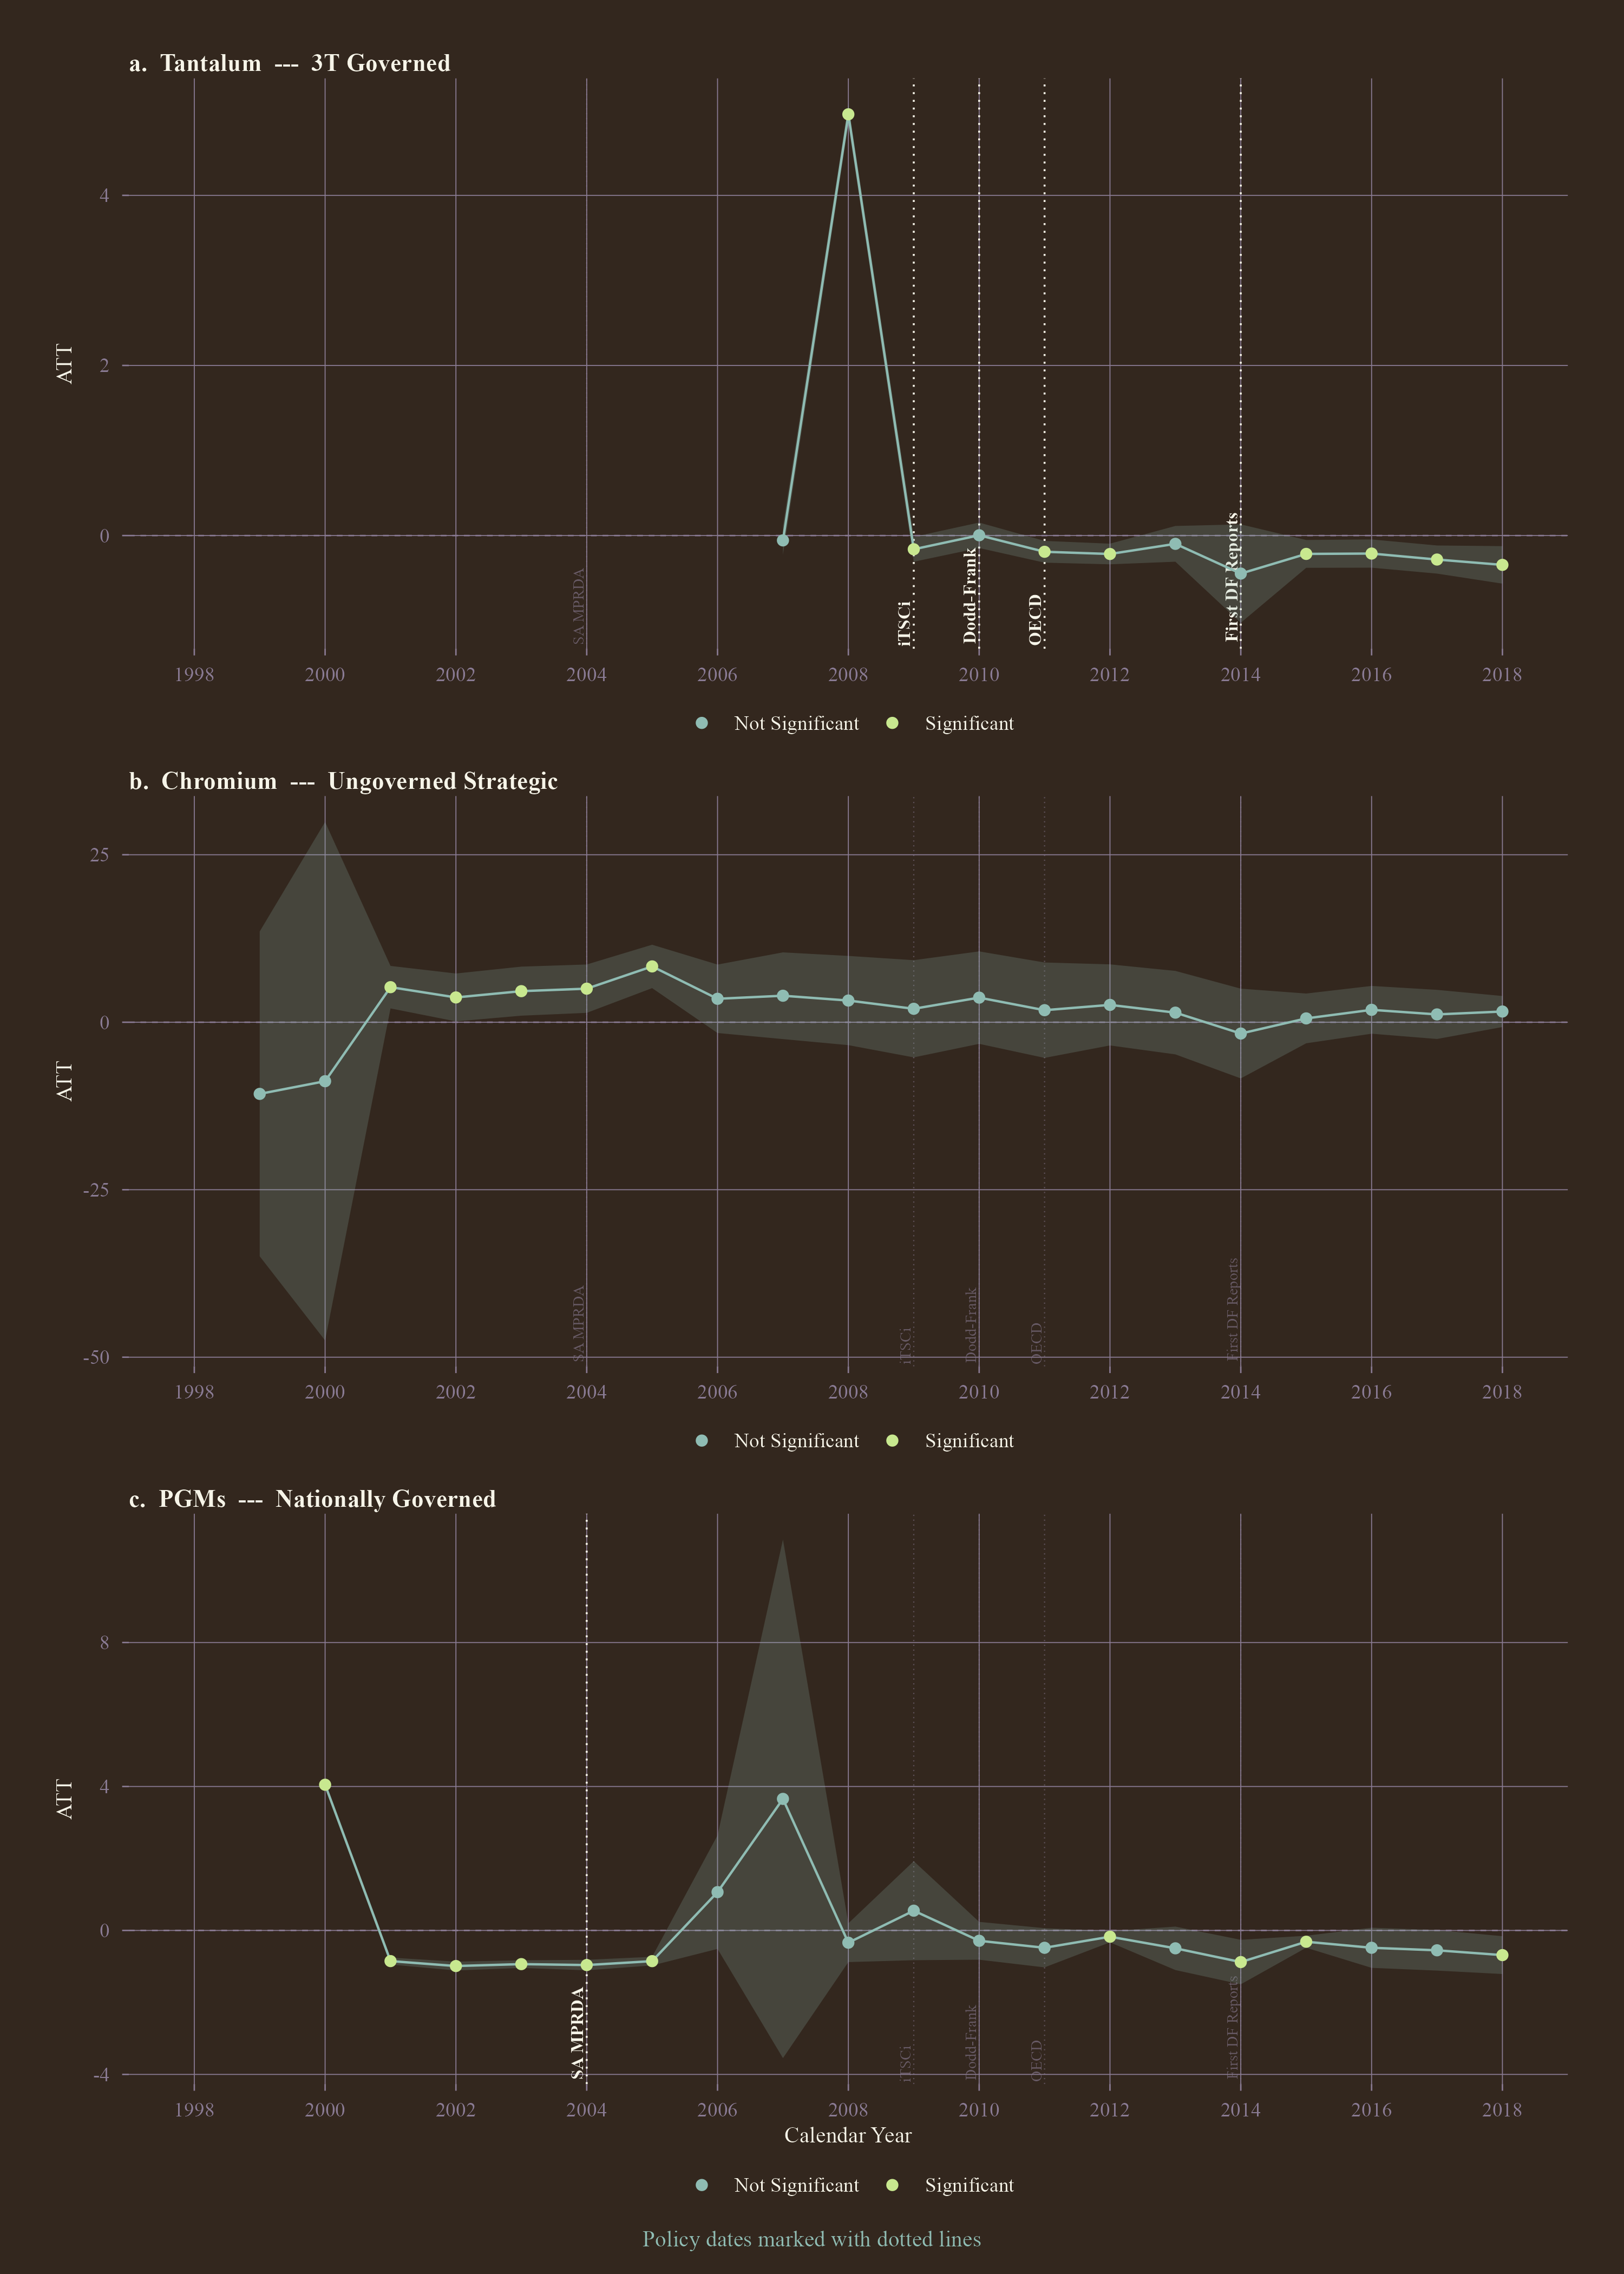
\includegraphics[width=0.8\textwidth]{plots/all_minerals_calendar_comparison.png}
    \caption{Calendar-time event studies aligned to policy milestones. Vertical lines mark key governance interventions, namely SA MPRDA (2004), iTSCi (2009), Dodd-Frank (2010), OECD guidelines (2011), and first Dodd-Frank reports (2014). Panel (a) shows tantalum (3T governed) with declining conflict after Dodd-Frank. Panel (b) shows chromium (governance gap) with increased battle deaths and no policy triggers. Panel (c) shows PGMs (nationally governed) with gradual decline beginning after MPRDA. See Tables~\ref{tab:cal_tantalum}, \ref{tab:cal_chromium}, and \ref{tab:cal_pgms} for full estimates.}
    \label{fig:calendar}
\end{figure}

\subsection{Mechanisms: Actor-Level Decomposition}
\label{sec:mechanisms}

% [PL C282] Rewritten opener. The ambiguous "who is affected" framing is replaced
% with the initiator/target distinction defined in Section 3.1.
The aggregate results establish that governance structure shapes the mineral-conflict relationship, but they treat all violence as equivalent. They cannot say which kinds of actors are doing the killing, or which are being killed. We address this by decomposing conflict outcomes by actor type and role using the UCDP Actor Dataset (v25.1), following the initiator and target definitions set out in Section \ref{sec:data}. For each mineral we estimate separate event-study models for formal armed group activity, both as initiators and as targets, for state-initiated violence, and for the targeting of civilians.

The set of actor outcomes varies by mineral depending on data availability. Formal armed groups show no variation in treated hexagons for tantalum and chromium at 100km, meaning too few treated units record any formal group activity at all, so these minerals support only state and civilian outcomes. PGMs, which have richer conflict data in treated hexagons, support estimation across all actor types.

\subsubsection{Tantalum: Universal Pacification}

Figure \ref{fig:mech_tantalum} presents the actor-level decomposition for tantalum. Under international governance, all estimable actor outcomes decline.

\begin{figure}[H]
    \centering
    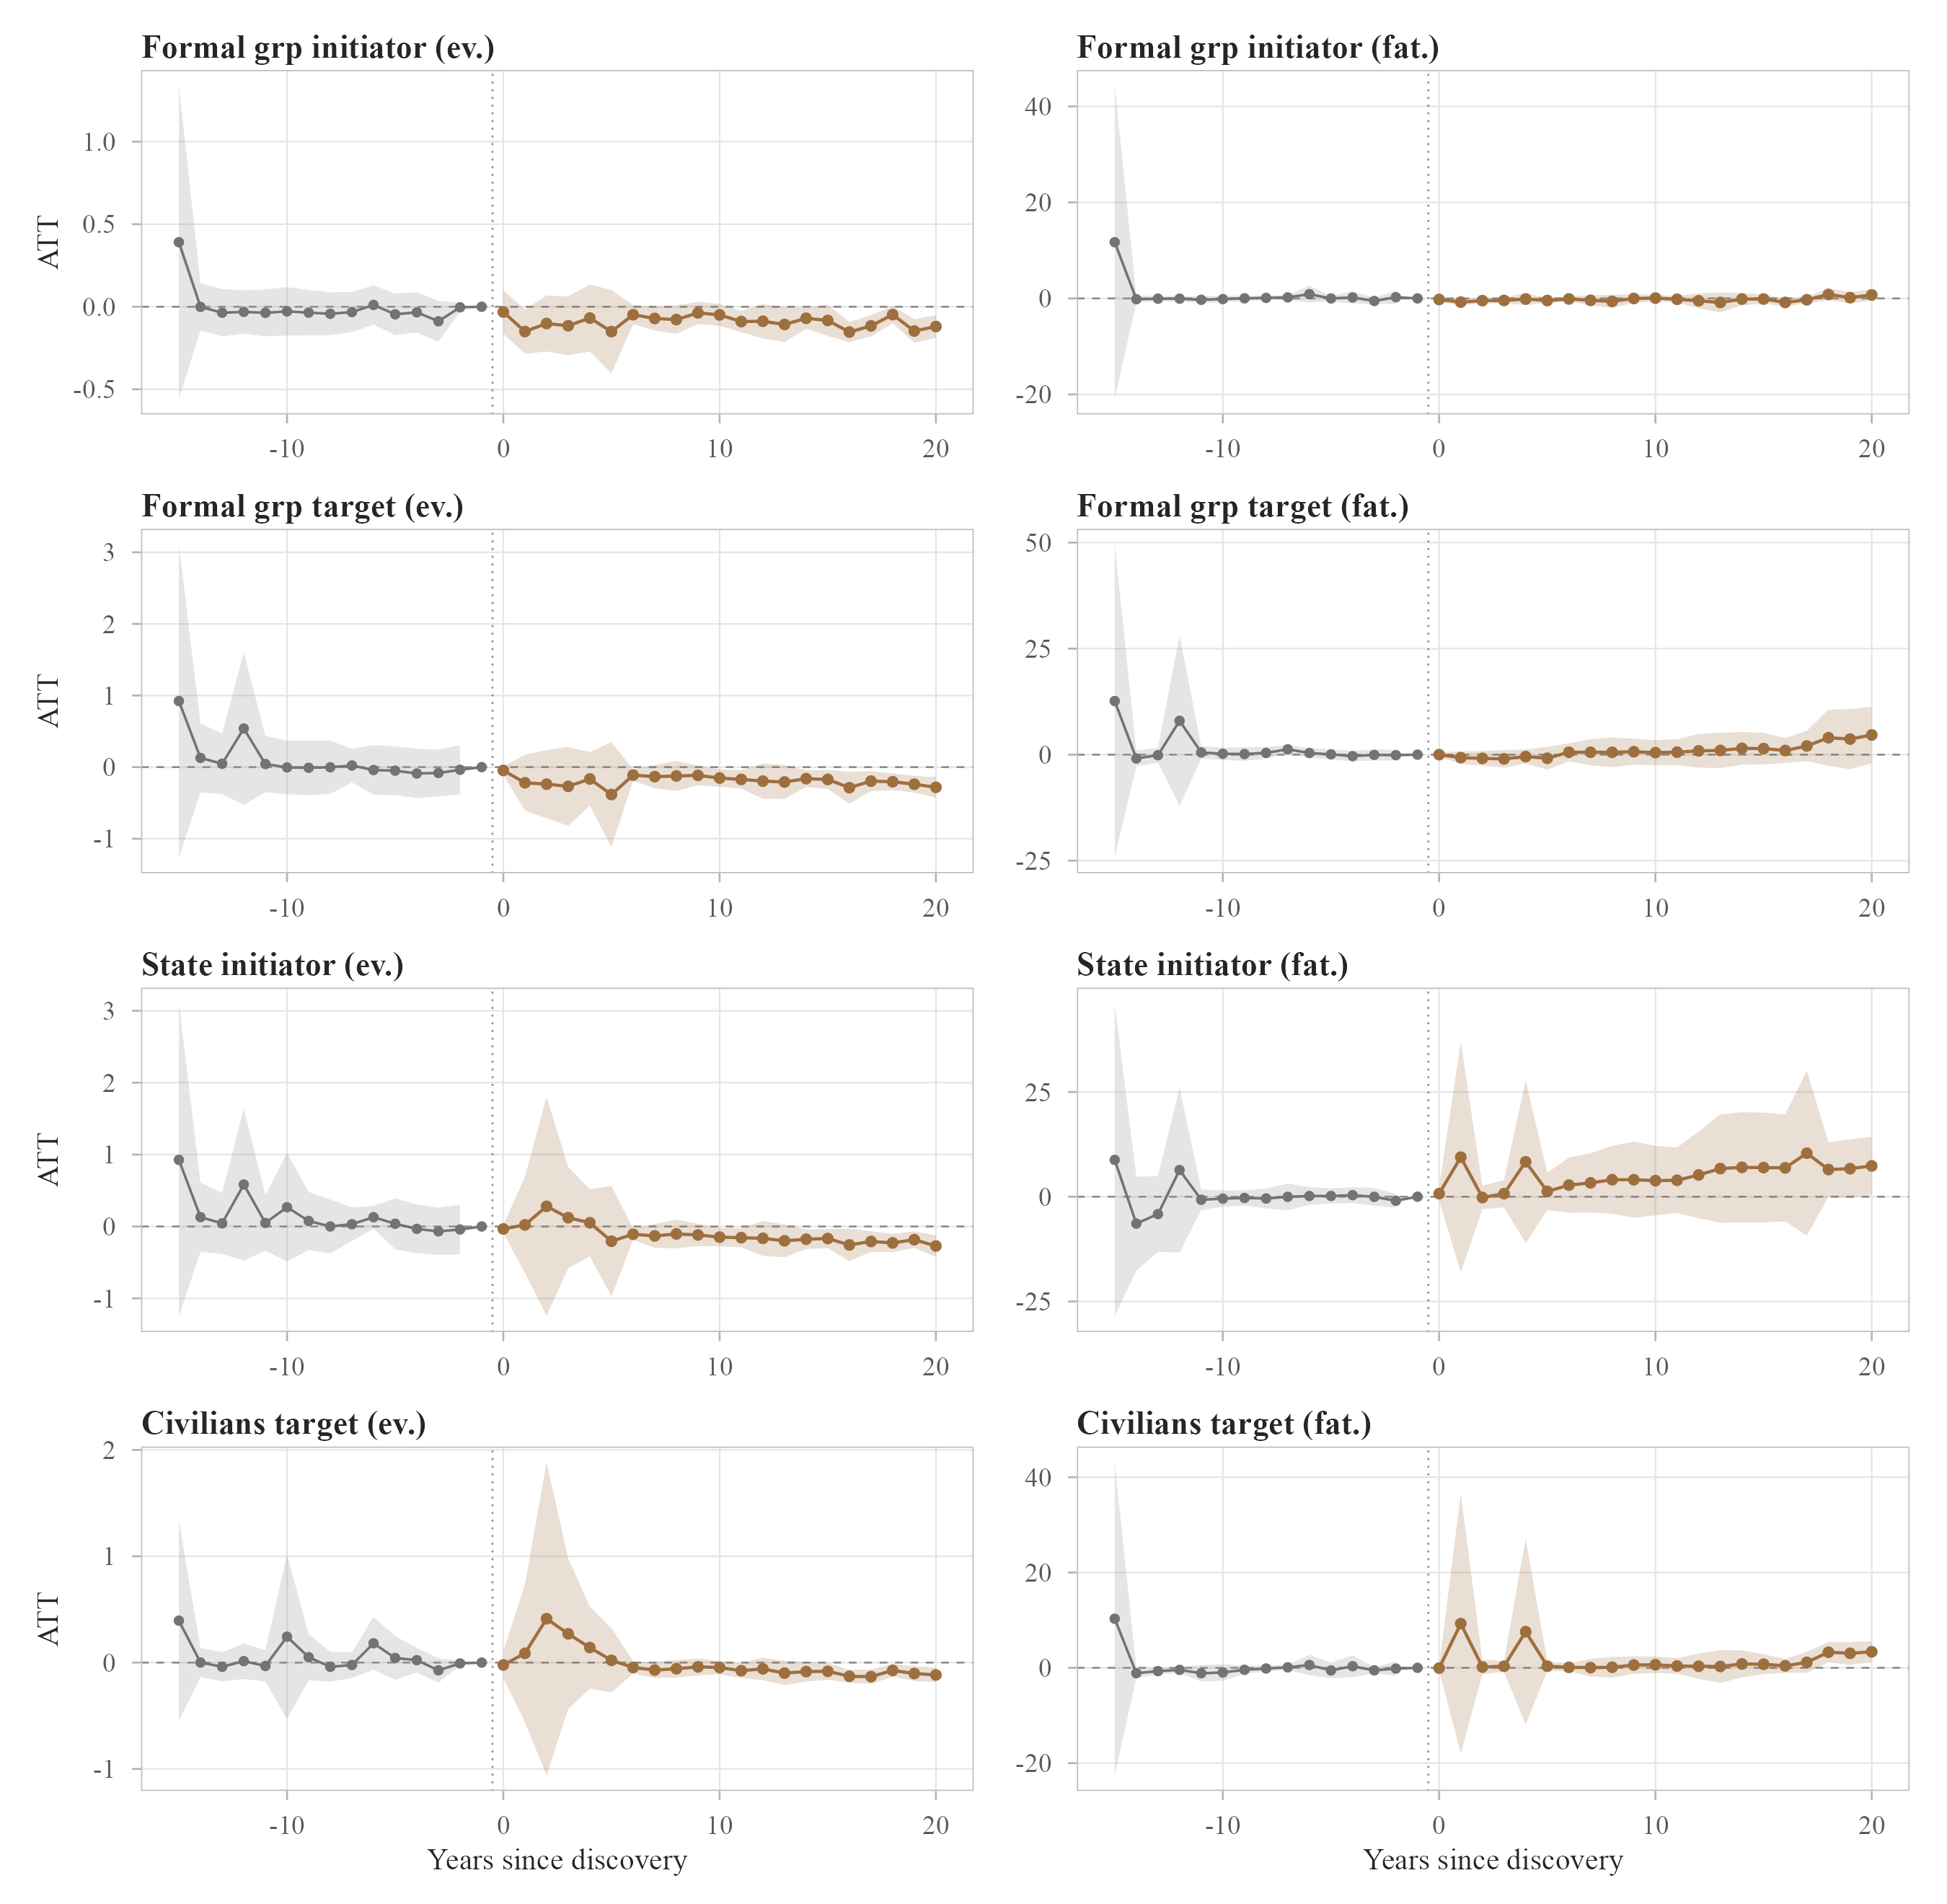
\includegraphics[width=0.95\textwidth]{plots/mechanism_tantalum_actors.png}
    \caption{Actor-level mechanism for tantalum (3T governed, 100km). State-initiated fatalities decline significantly (8 significant post-treatment periods). Civilian targeting, both events and fatalities, declines (8 and 5 significant periods respectively). Formal armed groups have no variation in treated hexagons and so cannot be estimated.}
    \label{fig:mech_tantalum}
\end{figure}

State-initiated fatalities show a sustained decline following tantalum discovery, with 8 significant post-treatment periods. The targeting of civilians declines in both frequency (8 significant periods) and lethality (5 significant periods). This broad pacification is consistent with international governance operating through supply chain transparency. By disrupting the revenue flows that sustain all parties to conflict, Dodd-Frank and related frameworks reduce violence regardless of which actors are involved. The pattern supports H1 and H2. See Table~\ref{tab:mech_tantalum} for full estimates.

\subsubsection{PGMs: Formal Group Exclusion Through State Monopoly}

For PGMs under national governance, the aggregate results show strong reductions in overall conflict events (Figure~\ref{fig:main_results}). The actor-level decomposition reveals the mechanism. Formal armed groups are systematically excluded from the conflict landscape around PGM deposits.

\begin{figure}[H]
    \centering
    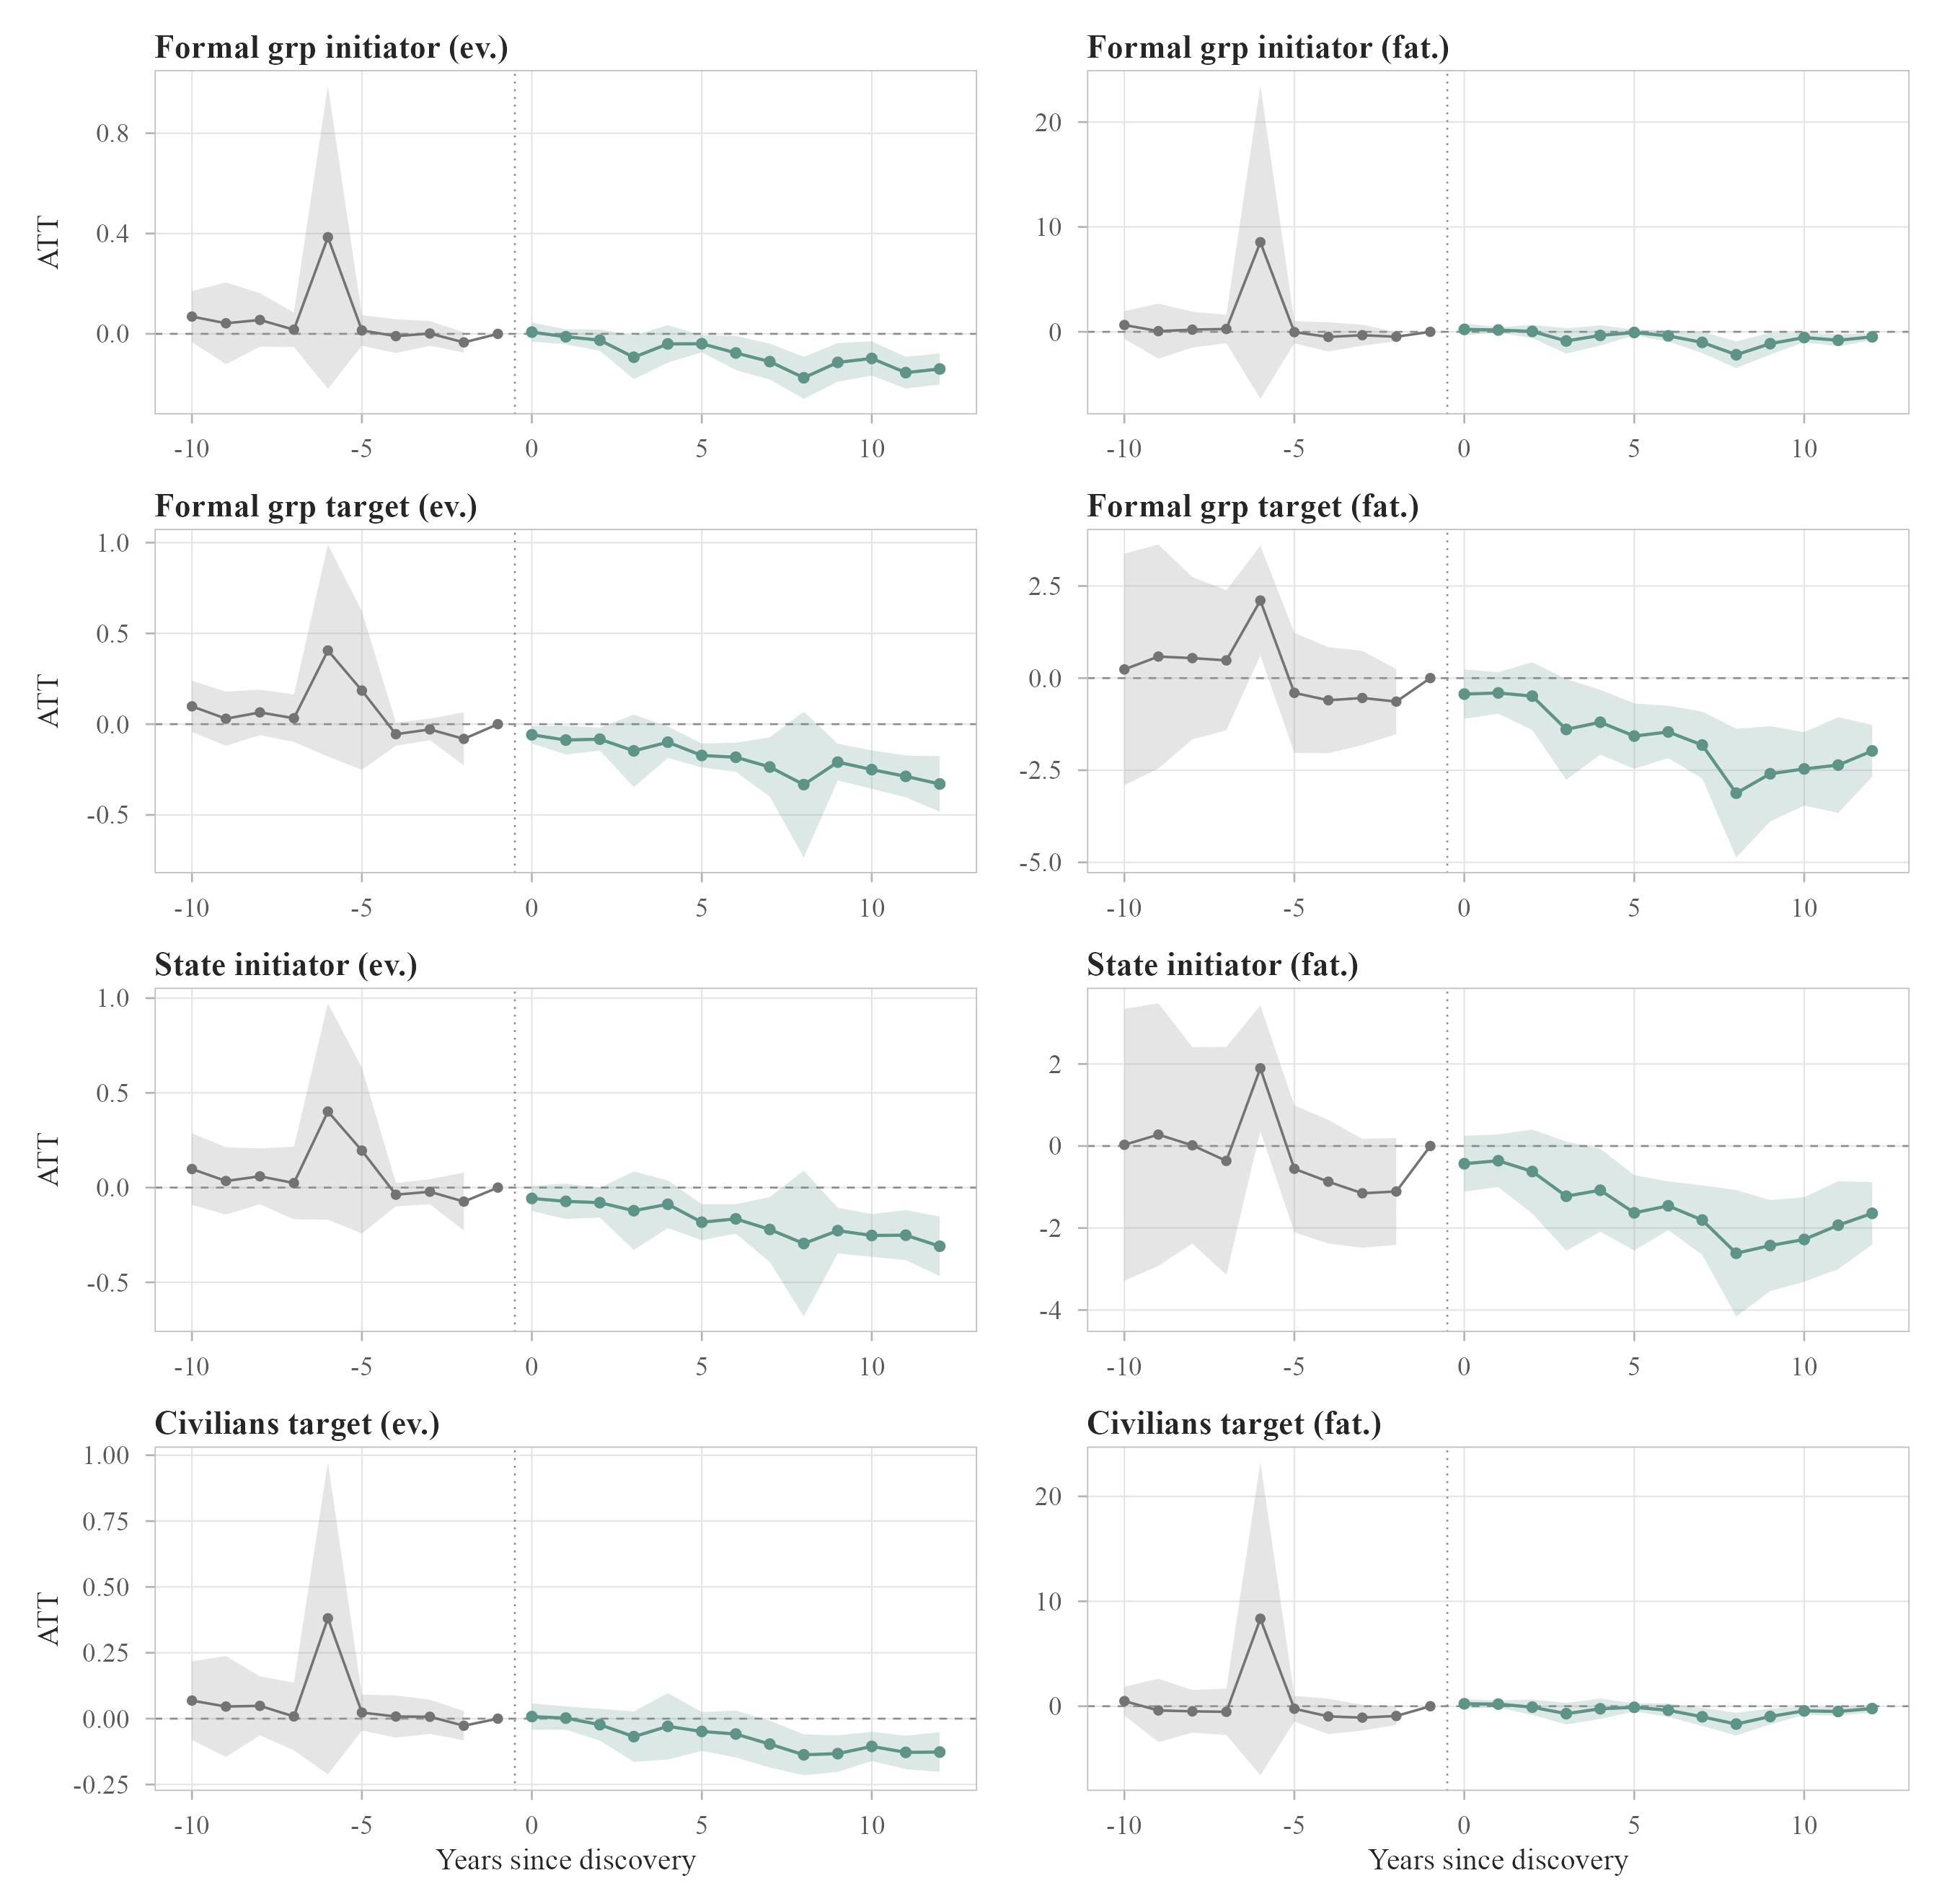
\includegraphics[width=0.95\textwidth]{plots/mechanism_pgms_actors.png}
    \caption{Actor-level mechanism for PGMs (nationally governed, 100km). Full decomposition across formal armed groups (as initiators and as targets), state actors, and civilians. The dominant pattern is the collapse of formal group-initiated fatalities (12 significant post-treatment periods, all negative). Formal groups as targets also decline. State-initiated and civilian-targeted outcomes show limited significant variation.}
    \label{fig:mech_pgms}
\end{figure}

The strongest result is the collapse of formal group-initiated fatalities, with 12 significant post-treatment periods showing negative effects, the most robust actor-level finding for any mineral. Formal armed groups are therefore killing far less around PGM deposits after discovery. They are also attacked less often, with formal groups as targets declining across 4 significant periods. By contrast, state-initiated and civilian-targeted outcomes show no significant post-treatment effects, indicating that national governance operates on organized challengers to extraction rather than suppressing all violence uniformly. This selective exclusion is consistent with H3. The state's monopoly over PGM extraction makes it unprofitable and dangerous for formal armed groups to contest access, while state and civilian outcomes remain largely unaffected. See Table~\ref{tab:mech_pgms} for full estimates.

\subsubsection{Chromium: State Lethality and the Decoupling Mechanism}

Figure \ref{fig:mech_chromium} shows the actor-level mechanism underlying chromium's decoupling pattern.

\begin{figure}[H]
    \centering
    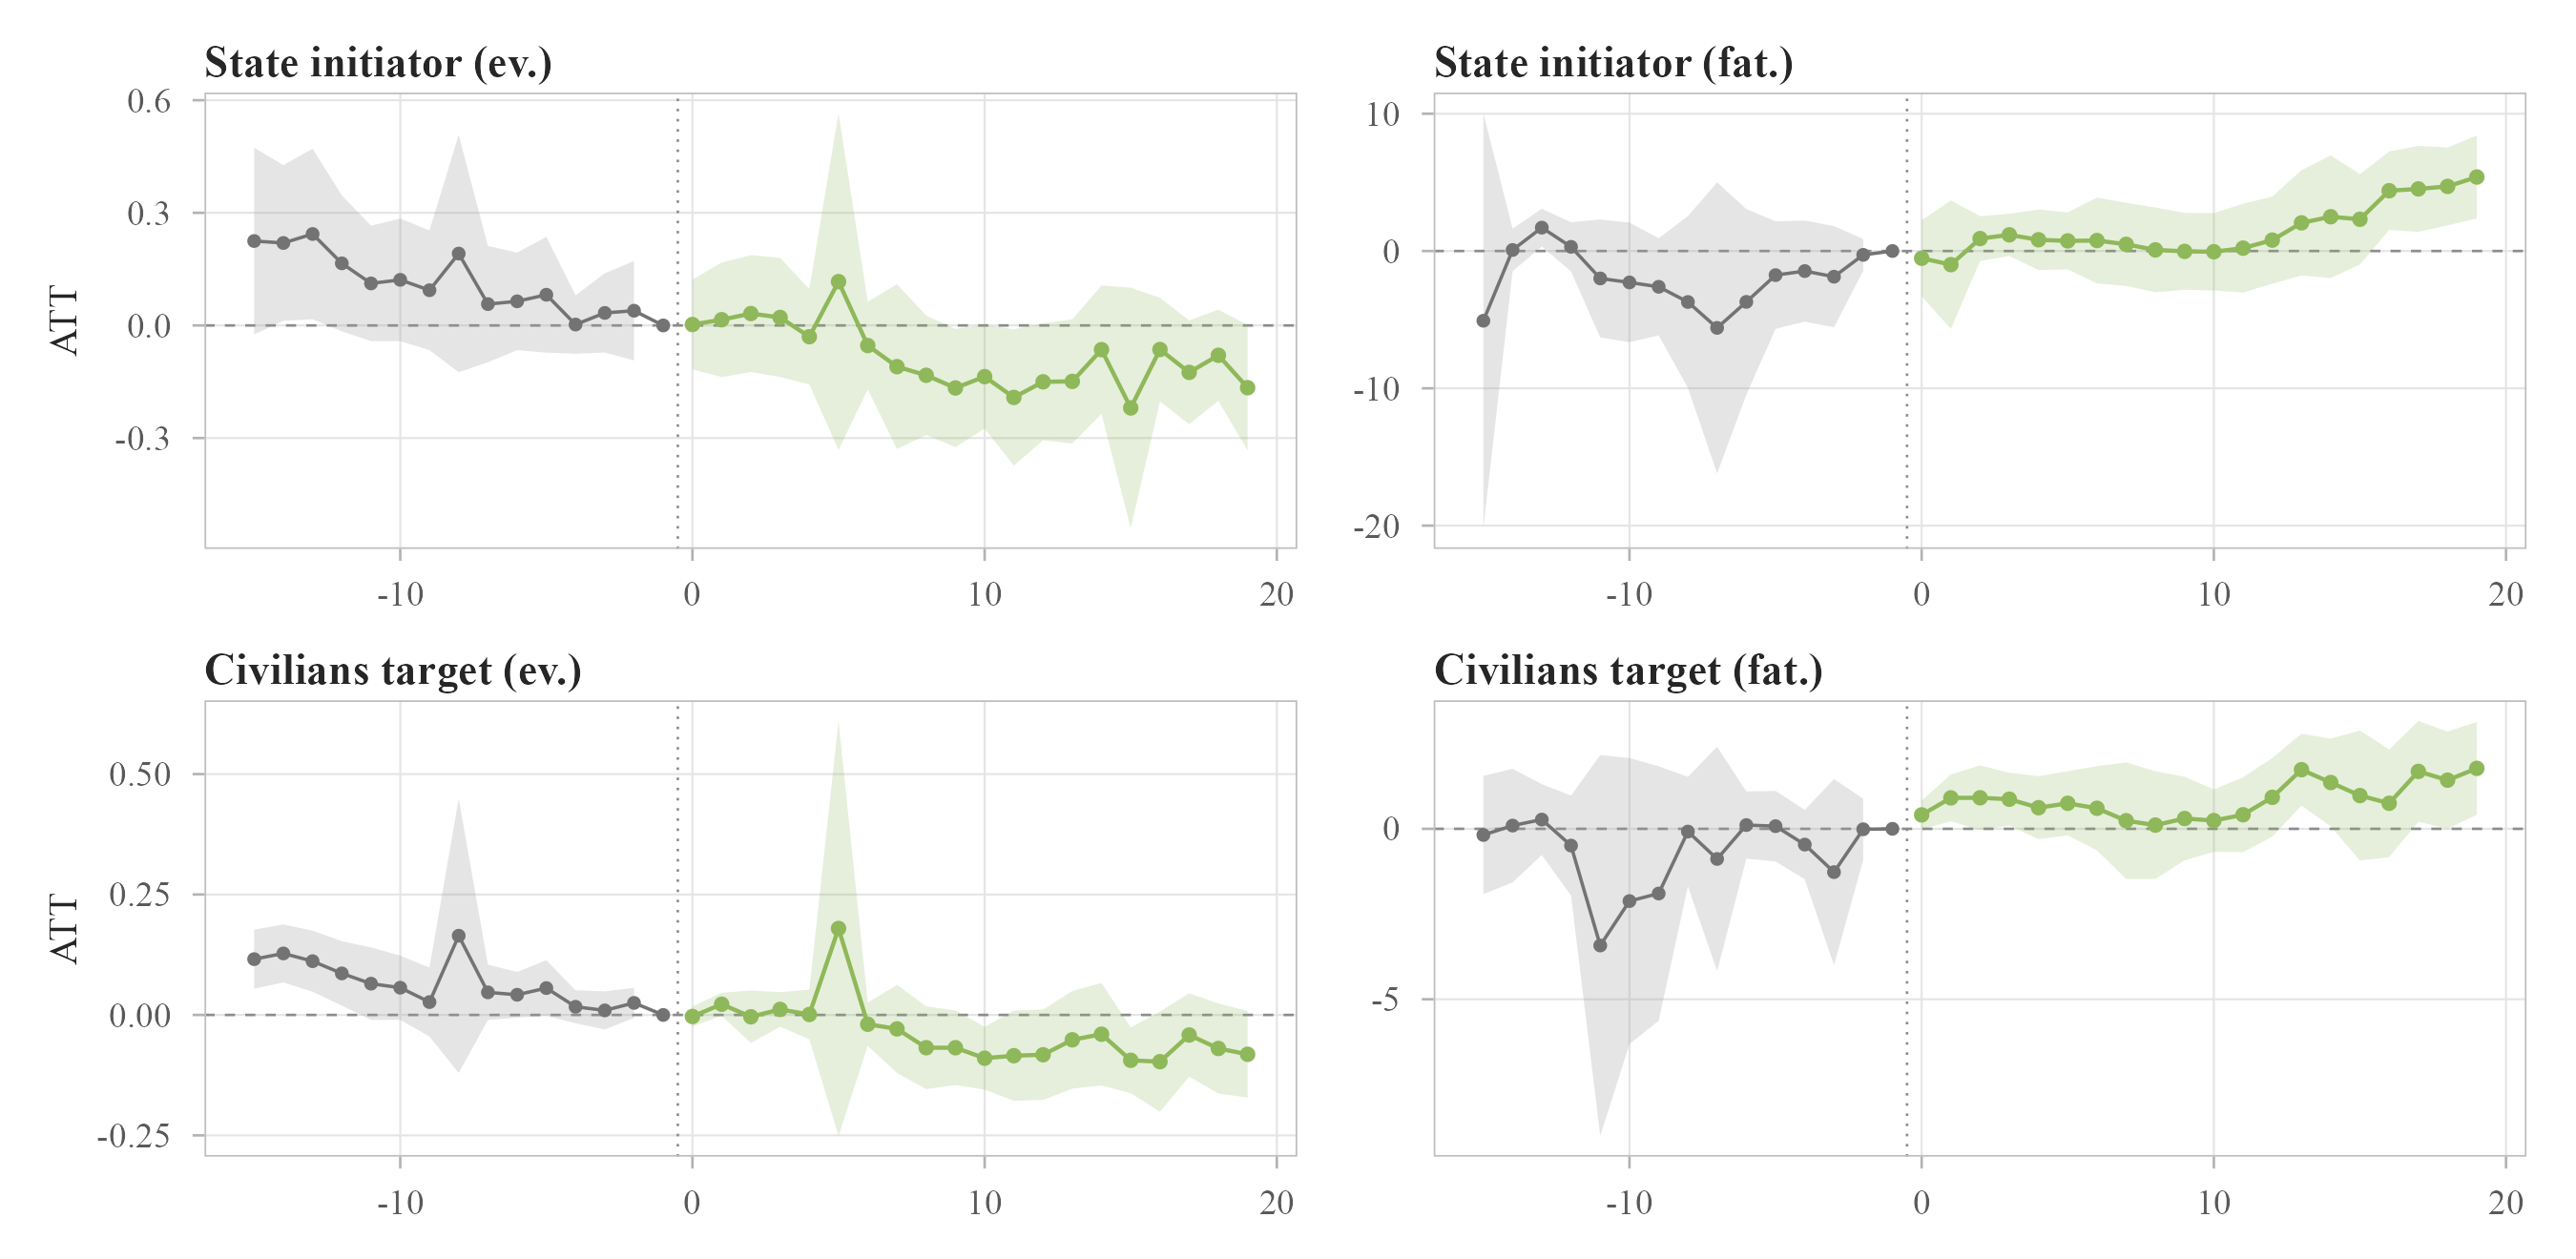
\includegraphics[width=0.95\textwidth]{plots/mechanism_chromium_actors.png}
    \caption{Actor-level mechanism for chromium (ungoverned strategic, 100km). State-initiated fatalities increase significantly (7 significant post-treatment periods, positive). Civilian fatalities increase (5 significant periods, positive). Formal armed groups are entirely absent, with no variation in treated hexagons.}
    \label{fig:mech_chromium}
\end{figure}

State-initiated fatalities increase following chromium discovery, with 7 significant post-treatment periods showing positive effects. Civilian fatalities also increase, across 5 significant periods. Formal armed groups, meanwhile, are entirely absent from chromium-adjacent hexagons at 100km. There is no variation in formal group activity to estimate, indicating that these groups simply do not operate near chromium deposits. That absence is itself informative. Chromium extraction is industrial rather than artisanal, so it offers armed groups none of the dispersed revenue opportunities available around 3T deposits, and there is no certification regime whose capture would be worth contesting.

The decoupling mechanism therefore operates as follows. Chromium's strategic value draws state forces to secure deposits, but the absence of governance frameworks means this securitization occurs without transparency requirements, conflict-free certification, or international oversight. The result is increased state-initiated lethality and civilian casualties, a ``security paradox'' in which state presence raises deaths rather than reducing them. This supports H5 and identifies the actors driving the decoupling pattern. See Table~\ref{tab:mech_chromium} for full estimates.

\subsubsection{Mechanism Summary}

Table \ref{tab:mech_combined} summarizes the actor-level findings across governance tiers. The pattern is systematic.

\begin{itemize}
    \item \textbf{International governance (tantalum).} All estimable actor outcomes decline. State-initiated fatalities down, events targeting civilians down, civilian fatalities down.
    \item \textbf{National governance (PGMs).} Formal groups excluded both as initiators (12 significant periods) and as targets. State and civilian outcomes unaffected. State monopoly control operates on organized challengers.
    \item \textbf{Governance gap (chromium).} Formal groups absent, but state lethality increases and civilians bear the cost. Governance gaps do not mean the absence of state actors. They mean the absence of \textit{constraints} on state actors.
\end{itemize}

% [PL C282] Key added below the table so the Actor Outcome abbreviations and the
% distinction between the Dir and ATT columns are legible without the R code.
\begin{table}[H]
\centering
\footnotesize
\caption{Actor-level effects of mineral discovery by governance tier (100\,km, never-treated controls)}
\label{tab:mech_combined}
\begin{tabular}{lllrrr}
\toprule
\textbf{Mineral} & \textbf{Tier} & \textbf{Actor outcome} & \textbf{ATT} & \textbf{ATT ($e\geq10$)} & \textbf{Pre} \\
\midrule
Tantalum & International & Formal grp initiator (ev.) & -0.092$^{***}$ (0.027) & -0.097$^{***}$ (0.029) & 1 \\
 &  & Formal grp initiator (fat.) & -0.221 (0.291) & -0.099 (0.395) & 0 \\
 &  & Formal grp target (ev.) & -0.194$^{***}$ (0.071) & -0.206$^{***}$ (0.061) & 1 \\
 &  & State initiator (fat.) & 5.042 (3.187) & 6.493 (4.733) & 0 \\
 &  & Civilians target (fat.) & 1.570$^{*}$ (0.808) & 1.315 (0.917) & 0 \\
\midrule
PGMs & National & Formal grp initiator (ev.) & -0.249 (0.206) & -0.329 (0.236) & 2 \\
 &  & Formal grp initiator (fat.) & -0.440 (0.465) & -0.473 (0.583) & 1 \\
 &  & Formal grp target (ev.) & -0.112$^{*}$ (0.062) & -0.185$^{***}$ (0.060) & 2 \\
 &  & State initiator (fat.) & 8.853 (5.734) & 9.993 (6.899) & 1 \\
 &  & Civilians target (fat.) & 2.466 (1.579) & 1.650 (1.285) & 0 \\
\midrule
Chromium & Governance gap & Formal grp initiator (ev.) & \multicolumn{3}{c}{\textit{no activity in treated cells}} \\
 &  & Formal grp target (ev.) & \multicolumn{3}{c}{\textit{no activity in treated cells}} \\
 &  & State initiator (fat.) & 1.512 (0.942) & 2.681$^{**}$ (1.227) & 0 \\
 &  & Civilians target (fat.) & 0.850$^{**}$ (0.431) & 1.128$^{**}$ (0.541) & 0 \\
\bottomrule
\end{tabular}
\begin{minipage}{0.95\textwidth}\vspace{4pt}\scriptsize
\textit{Notes.} \textit{Initiator} denotes the side that carried out the violence and \textit{target} the side against which it was directed. ``ev.'' is a count of events, ``fat.'' a count of battle deaths. \textbf{ATT} is the dynamic Callaway--Sant'Anna aggregate across all post-treatment periods; \textbf{ATT ($e\geq10$)} the average from the tenth post-treatment year, identified from the earliest discovery cohorts only. Standard errors in parentheses. \textbf{Pre} counts pre-treatment coefficients falling outside the estimator's simultaneous confidence band. Treated cells: tantalum 25, PGMs 8, chromium 11. $^{*}p<0.10$, $^{**}p<0.05$, $^{***}p<0.01$.
\end{minipage}
\end{table}


\noindent\footnotesize In the Actor Outcome column, \textit{initiator} denotes the side that carried out the violence and \textit{target} the side against which it was directed, following the definitions in Section \ref{sec:data}. ``ev.'' denotes a count of events and ``fat.'' a count of battle deaths. \textit{Sig Post} and \textit{Sig Pre} count the individual post- and pre-treatment period coefficients significant at $p<0.05$. \textit{Dir} reports the sign of the significant post-treatment coefficients only, whereas \textit{ATT} is the simple Callaway-Sant'Anna aggregate over all post-treatment periods. The two columns therefore answer different questions and need not agree in sign. \normalsize

% [PL C295] PL proposed reporting platinum only here and dropping copper and
% cobalt as minerals not used elsewhere in the paper. Not applied. Copper and
% cobalt are the only two production-onset results with flat pre-trends and
% significant effects, while the PGM estimates fail pre-trends and are already
% reported as descriptive only, so a platinum-only section would report nothing
% interpretable. Raised with PL rather than actioned unilaterally.
\section{Robustness: Production Onset as Treatment}
\label{sec:production}

We re-estimate the design using the start of mineral production as the
treatment in place of the discovery year, drawing treatment dates from the
Open Database on Mine Production (the recorded production-start year for each
African facility, or its first reported output year where no start year is
given). The grid, outcomes, and estimator are unchanged. Three critical
minerals carry enough producing facilities for estimation, namely copper,
cobalt, and platinum-group metals (PGMs). The 3T group (tantalum, tin, tungsten) is
absent from the industrial-production data, so this test cannot speak to it.

Copper gives the clearest result. Across 17 treated hexes with flat
pre-trends, production onset lowers the local count of conflict events
(Table~\ref{tab:prod_results}, Appendix Figure~\ref{fig:prod_copper}). Cobalt points
the same way on a smaller base of 7 hexes, which is reassuring given that
regional cobalt is mined as a copper by-product. For both minerals the effect
is on the frequency of events, not on battle deaths, which remain a noisy
zero. The PGM hexes sit on a rising-conflict path before their recorded start
years and several pre-treatment leads are significant, so we read those
estimates as descriptive only. The production design marks a different moment
in a mine's life than discovery and covers only industrial operations, so we
treat it as a separate test of a production-onset mechanism, not a
replication of the discovery findings. Appendix~\ref{ap:prod_figs} presents the
event-study figures for all three minerals.

\begin{table}[htbp]
\centering
\caption{Production-onset effects on local conflict (100\,km, not-yet-treated controls)}
\label{tab:prod_results}
\begin{tabular}{llrrrc}
\toprule
\textbf{Mineral} & \textbf{Outcome} & \textbf{Treated hexes} & \textbf{ATT} & \textbf{SE} & \textbf{Pre-trends} \\
\midrule
Copper & Conflict events & 17 & $-0.208$ & 0.053 & flat \\
Copper & Battle deaths   & 17 & $1.016$  & 2.440 & flat \\
Cobalt & Conflict events &  7 & $-0.224$ & 0.064 & flat \\
Cobalt & Battle deaths   &  7 & $0.110$  & 1.184 & flat \\
PGMs   & Conflict events &  8 & $-0.049$ & 0.112 & violated \\
PGMs   & Battle deaths   &  8 & $1.441$  & 0.646 & violated \\
\bottomrule
\end{tabular}
\\[4pt]
{\footnotesize ATT is the simple aggregate Callaway--Sant'Anna estimate. Copper
and cobalt conflict-event effects are significant at the 1\% level.}
\end{table}

\noindent The event-study figures for these estimates appear in Appendix~\ref{ap:prod_figs}.


\subsection{Limitations}

% [ED C308 / PL C255] Both authors asked for this to be toned down. PL cut the
% long 2018-cutoff passage and the production-onset paragraph, and flattened the
% subsections into continuous prose.
Our analysis provides a starting point for understanding how governance mediates the mineral-conflict relationship, but several limitations warrant discussion.

Our identification strategy relies on mineral discovery as the treatment, capturing the moment when a location's resource potential becomes known. This approach offers identification advantages because discovery timing is plausibly exogenous to local conflict dynamics, and it allows us to estimate anticipatory effects before extraction begins. However, discovery and active mining likely operate through different mechanisms. Discovery may trigger conflict through expectations of future wealth, speculative land grabs, and positioning by armed groups seeking to control eventual extraction \citep{cust2015dutch, lei2019natural}. Mining, by contrast, generates actual revenue flows, employment, infrastructure development, and sustained interactions between extractive firms, state authorities, and local communities. The development channel of roads, jobs, and services that accompanies active mining could either amplify pacification, through opportunity costs of violence and improved state capacity, or intensify conflict, through grievances over distribution, environmental damage, and displacement \citep{aragon2015mining, kotsadam2018industrial}. There are no publicly available datasets on critical minerals production.

Alternative mechanisms could generate patterns consistent with our findings, and we cannot fully isolate among them with the current design. The decoupling pattern for chromium could reflect not governance gaps but geological characteristics. Chromium deposits are often associated with large-scale industrial mining operations, concentrating extraction in facilities less susceptible to artisanal mining but potentially more attractive as targets for state securitization. Disentangling governance from geology requires within-mineral variation in institutional frameworks that does not yet exist for chromium. Further, the pacification effects we attribute to Dodd-Frank and related frameworks could instead reflect broader trends in the regions where governed minerals are located. The eastern DRC, for instance, experienced significant international peacekeeping expansion and security sector reform during our study period. While our difference-in-differences design with cell fixed effects absorbs time-invariant regional characteristics, it cannot fully rule out confounding from spatially targeted interventions that coincided with governance implementation.

Several measurement issues merit acknowledgment. Battle death estimates from UCDP carry considerable uncertainty, particularly for events in remote areas with limited reporting infrastructure. Our reliance on the best estimate may obscure important variation, and the wide confidence intervals on lethality effects partly reflect this. We use a variety of spatial scales in the robustness appendix to further parse the spatial precision of these effects. Our mineral discovery data capture documented exploration-to-discovery activity reported to commercial databases, so informal discoveries, particularly of artisanally mined minerals, may go unrecorded. If informal discovery is correlated with conflict, either as cause or as consequence, our estimates could be biased. This concern is less acute for industrial minerals like PGMs and chromium and more relevant for minerals with artisanal potential. A further point concerns the temporal coverage of our data, which ends in 2018. The cutoff truncates follow-up length for the most recently discovered cohorts. Cells whose first discovery falls after 2018 are unobserved as treated and therefore sit in the never-treated comparison pool, which would attenuate our estimates if conflict around those cells already responds to exploration activity before the discovery is recorded.

Finally, the national governance findings rest entirely on a single country. South Africa holds the overwhelming majority of global platinum group metal reserves and output, and the PGM discoveries in our data are concentrated there. The exclusion of formal armed groups that we attribute to state monopoly control therefore reflects the specific institutional setting of South African mining, including the MPRDA and a state with the administrative reach to license and police industrial extraction. Whether national governance produces the same exclusion in settings with weaker state capacity or more contested territorial control is a question our data cannot answer. The PGM results are best read as evidence on how one strong national regulatory regime shapes mineral conflict, not as a general claim about national governance. This geographic concentration also makes the national governance tier less separable from country-level conditions than the other tiers, so its estimates warrant extra caution in any extrapolation beyond South Africa.

% [PL C80] PL asked whether the analysis should include only South African
% discoveries. Not applied pending her decision. Needs a count of non-SA PGM hexes.

\section{Discussion}
\label{sec:discussion}

Our findings have several implications for understanding the resource curse and for policy. Our results suggest that mineral wealth does not mechanically produce conflict \citep{ross2015resource, gilmore2005resource}. The same mineral that fueled violence in the DRC in the 1990s now shows pacifying effects following implementation of governance frameworks. This suggests the curse is not inherent to resource wealth but emerges from institutional failures that governance can address \citep{mehlum2006institutions, robinson2006governance}.

At the same time, governance gaps create new risks. The decoupling pattern we document for chromium represents a new and concerning dynamic. The actor-level decomposition identifies the mechanism. State forces become deadlier while formal armed groups are absent from the conflict landscape entirely. This is not the resource curse of the 1990s, where rebel groups competed for mineral rents. It is a pattern in which state securitization of strategically valuable deposits occurs without the transparency and accountability constraints imposed by international governance frameworks. As demand grows for minerals vital to clean energy and industrial infrastructure, the absence of governance frameworks may produce a new generation of ``blood minerals'' \citep{enough2009conflict}, but one driven by state violence rather than rebel predation.

Our results also indicate that different governance models suit different contexts. International frameworks, following the Dodd-Frank model, appear most effective for minerals with dispersed, artisanal extraction that can fund armed groups \citep{radley2021artisanal}. National governance, following the South African model, appears effective when industrial capacity requirements already exclude non-state actors. The mechanism analysis is consistent with this. International governance pacifies actors across the board through supply chain transparency, while national governance operates on formal armed groups through state monopoly control. Policy should match governance approach to extraction characteristics.

Anticipatory effects also matter. Our focus on discovery rather than production suggests that conflict dynamics shift before extraction begins \citep{cotet2013oil, arezki2017natural}. This has implications for early intervention. Governance frameworks should ideally be established before a mineral becomes strategically important, not after conflict patterns emerge.

\section{Concluding Remarks and Future Research}
\label{sec:conclusion}

The global energy transition will intensify demand for minerals concentrated in conflict-prone regions. This study shows that governance structure, and not mineral type alone, systematically conditions how critical mineral discoveries shape armed conflict in Africa. Our findings suggest this need not reproduce the resource conflicts of the past. Governance frameworks can break the link between mineral wealth and violence, as the pacifying effects of Dodd-Frank on 3T minerals demonstrate.

However, governance gaps pose serious risks. Chromium, currently lacking international frameworks, already shows the concerning pattern of increased state-initiated lethality and civilian casualties following discovery. The actor-level decomposition reveals that governance gaps do not simply leave a vacuum. They produce a distinctive conflict signature in which state forces securitize extraction sites without accountability, and civilians bear the cost. As chromium and similar minerals become more strategically important, extending governance frameworks could prevent escalation.

The policy implications of our study are actionable. Early, context-sensitive governance interventions at the discovery stage can prevent mineral wealth from becoming a source of violent competition. For minerals and regions that currently lack oversight, policymakers and industry should prioritize transparency, independent monitoring, and accountability measures to reduce the risk of securitization and civilian harm. Africa provides a key test case. The success of 3T governance shows that international cooperation can reshape conflict dynamics around extractive resources. The challenge now is extending that success to the critical minerals that will power the clean energy transition.

% [PL C388] Future-research material folded into this section, per PL's proposal.
Finally, the findings point to a research agenda with direct policy relevance. Future work should test whether the governance-contingent patterns documented here persist once production begins, and better firm-level and production data would sharpen causal inference and help translate supply-chain interventions into protections for communities living near strategic deposits. Spatial spillover analysis examining conflict dynamics in neighboring cells could help distinguish pacification from displacement, if governance frameworks push armed groups away from regulated minerals toward ungoverned alternatives \citep{berman2017spillover}. Other extensions include investigating how heterogeneity in country-level institutions relates to international governance frameworks. Dodd-Frank's effectiveness likely depends on baseline state capacity, rule of law, and integration into global supply chains, and cross-national variation in these factors could help identify scope conditions for governance-based interventions. Extending the analysis to other critical mineral frontiers, particularly Latin America and Southeast Asia, would test external validity. If governance-contingent effects replicate across continents with different colonial histories, state structures, and armed group configurations, confidence in the generalizability of our findings would increase. The emergence of new governance initiatives for battery minerals, cobalt in particular, also creates opportunities for prospective evaluation. Tracking conflict dynamics around cobalt deposits as frameworks like the Responsible Minerals Initiative expand coverage would provide quasi-experimental evidence on governance effects as they unfold.

\bibliography{bib}

\clearpage
\appendix
\renewcommand{\thetable}{\thesection\arabic{table}}
\renewcommand{\thefigure}{\thesection\arabic{figure}}
\setcounter{table}{0}
\setcounter{figure}{0}

\section{Robustness Across Spatial Scales}
\label{sec:scales}

Figure \ref{fig:africa_hex_grids} illustrates the hexagonal grid structure used for spatial aggregation at two resolutions. The 50km grid provides fine-grained local analysis, while the 300km grid captures broader regional patterns. Our main results (100km) fall between these extremes.

\begin{figure}[H]
    \centering
    \begin{subfigure}[b]{0.48\textwidth}
        \centering
        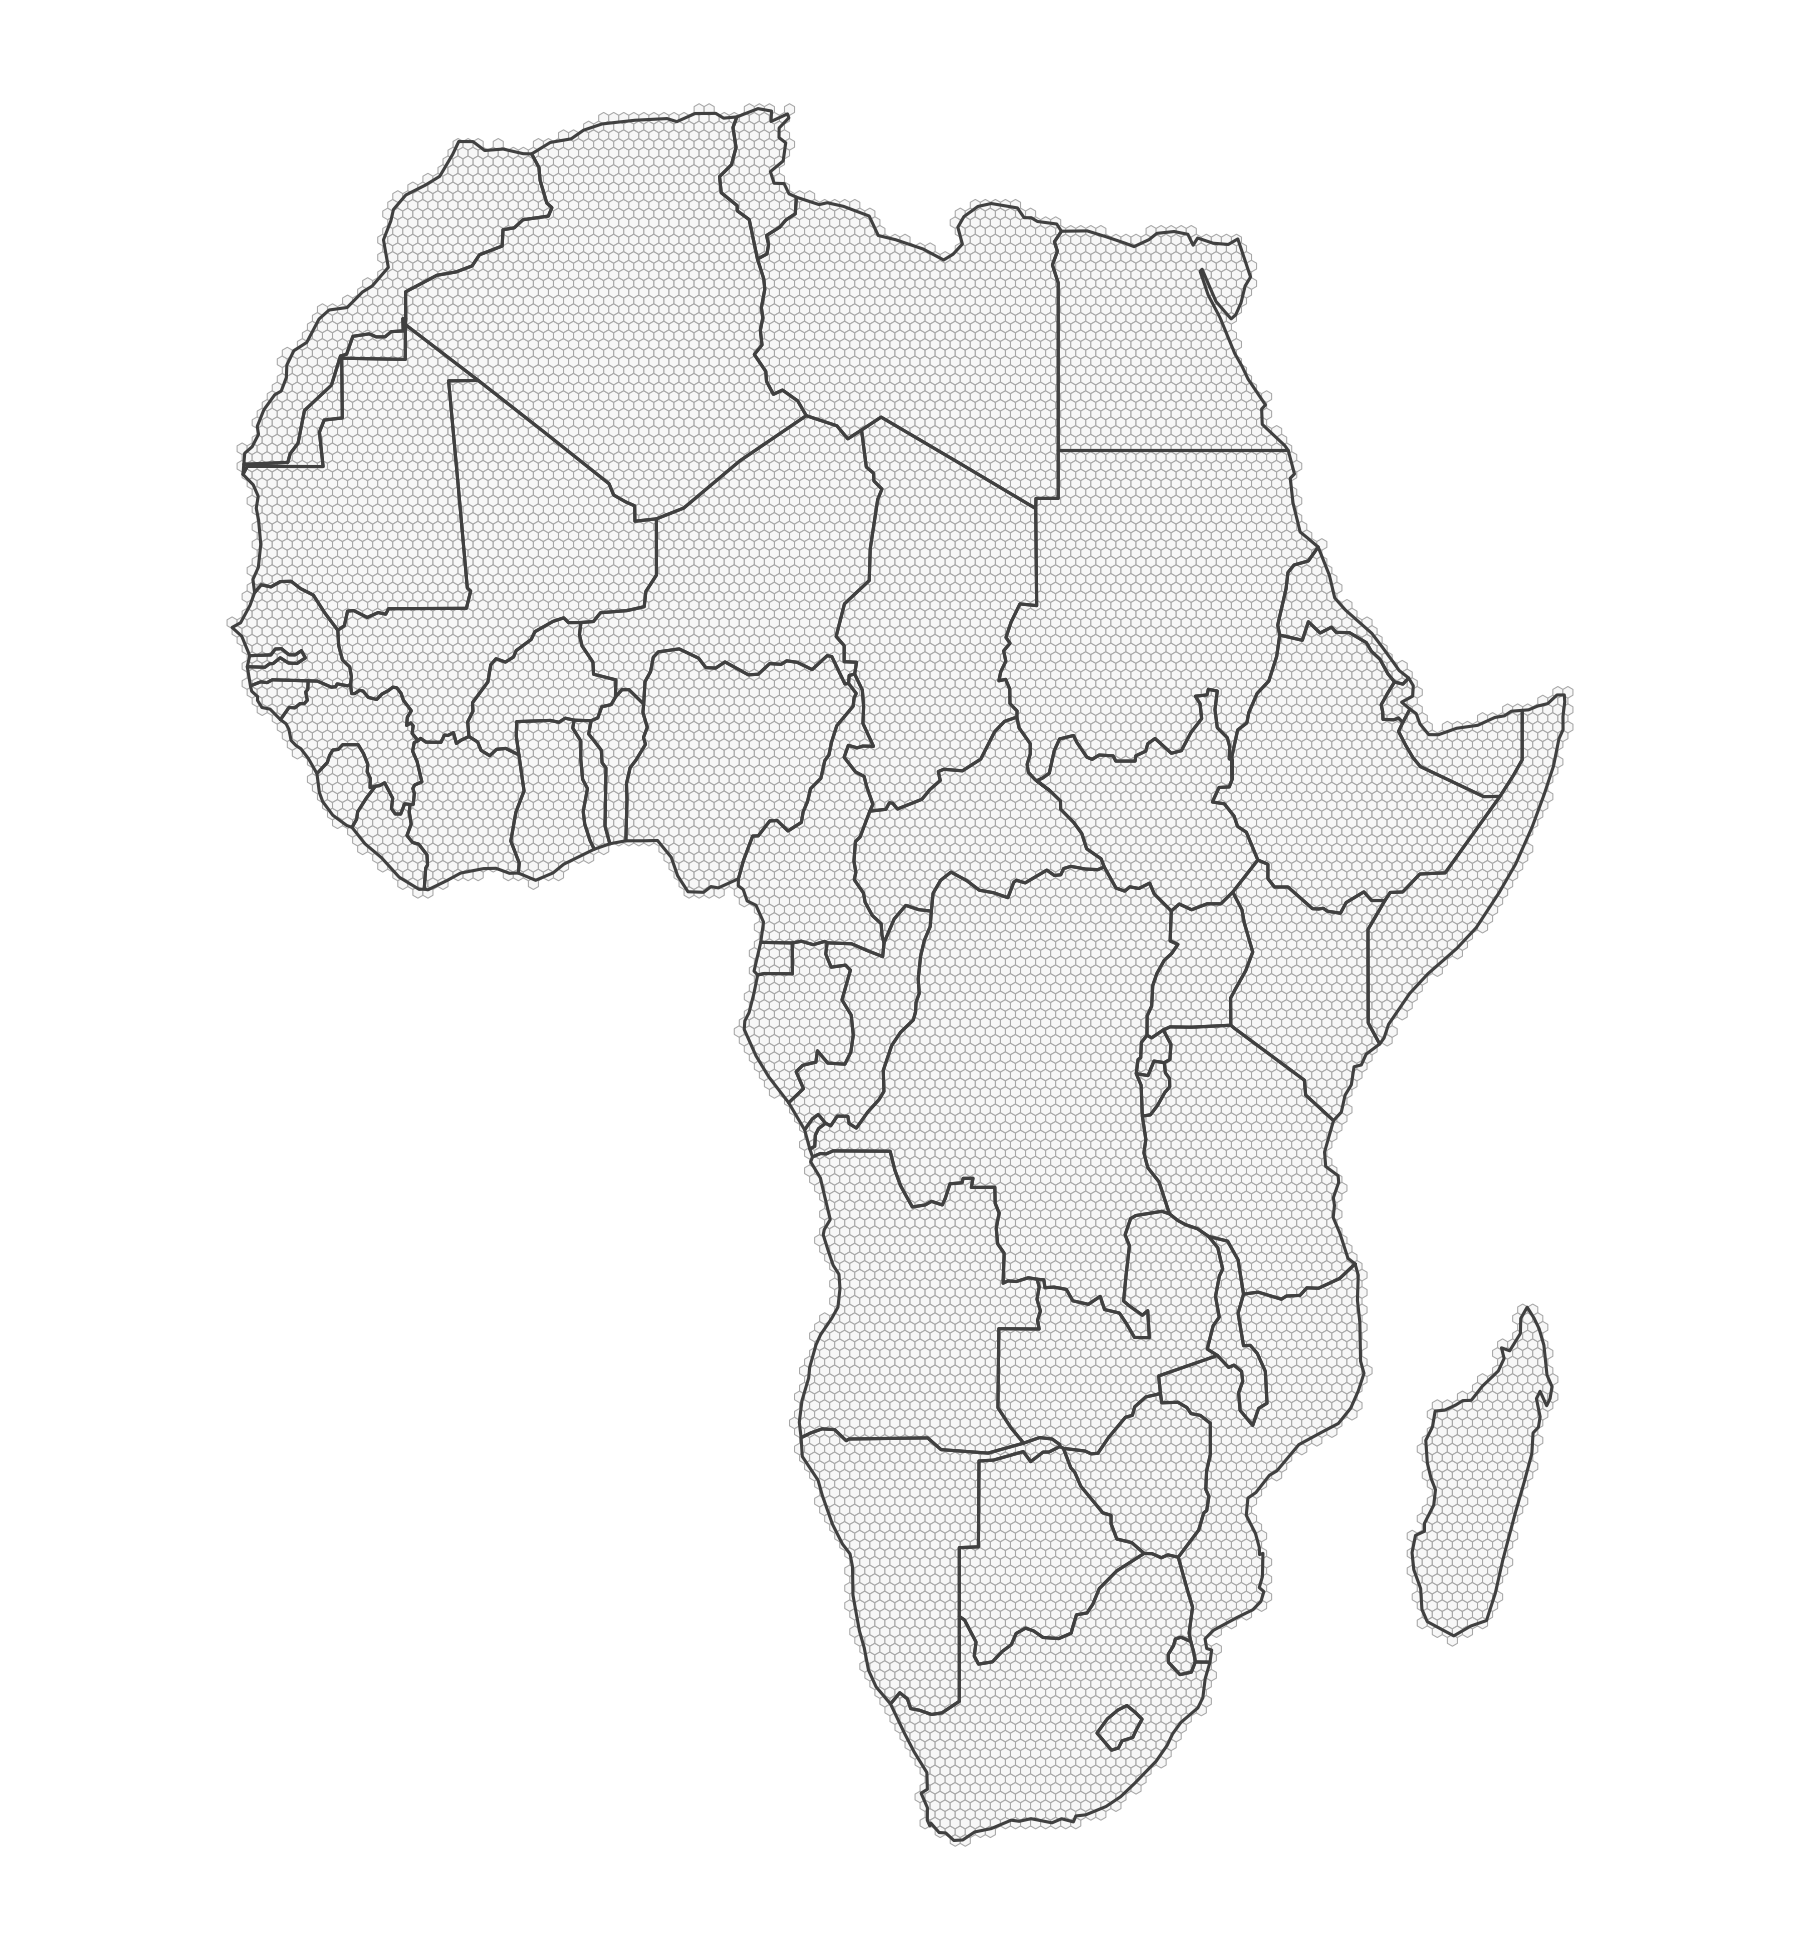
\includegraphics[width=\textwidth]{plots/Africa50km.png}
        \caption{50 km hex grid}
        \label{fig:africa50km}
    \end{subfigure}
    \hfill
    \begin{subfigure}[b]{0.48\textwidth}
        \centering
        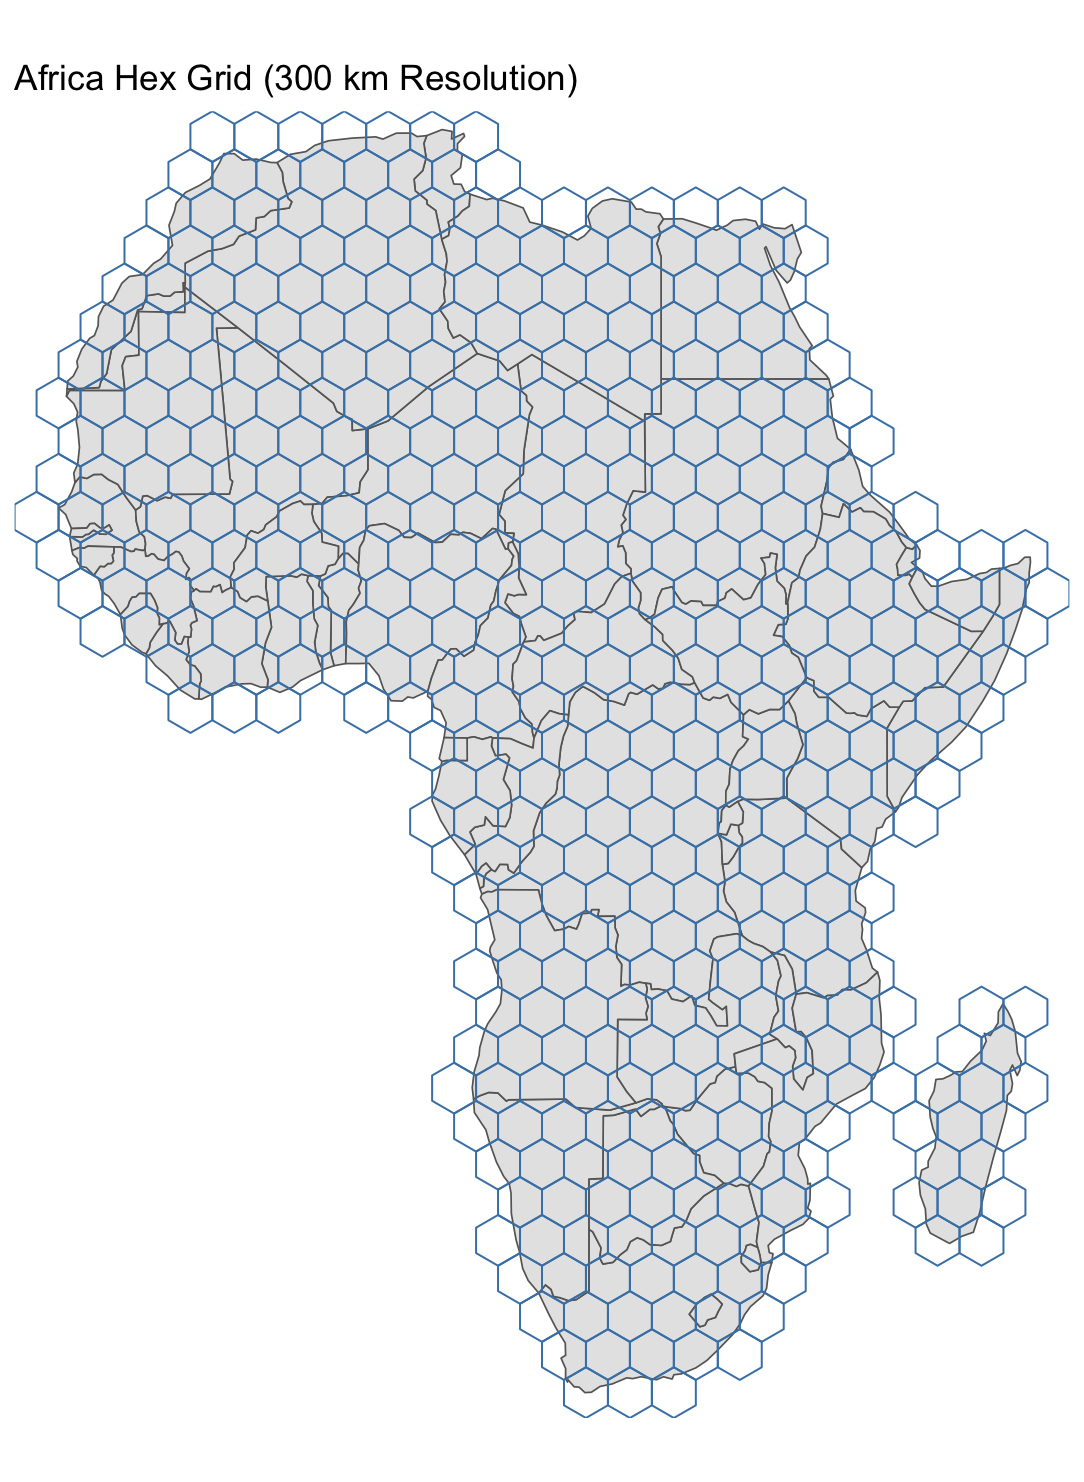
\includegraphics[width=\textwidth]{plots/Africa300km.png}
        \caption{300 km hex grid}
        \label{fig:africa300km}
    \end{subfigure}
    \caption{Africa hex grids at two resolutions. Left panel shows 50km diameter hexagons; right panel shows 300km diameter hexagons. Main analysis uses 100km resolution.}
    \label{fig:africa_hex_grids}
\end{figure}

\section{Production-Onset Robustness Figures}
\label{ap:prod_figs}
\setcounter{table}{0}
\setcounter{figure}{0}

These figures accompany the production-onset robustness analysis in Section~\ref{sec:production}. Each panel reports Callaway-Sant'Anna event-study estimates for conflict events (left) and battle deaths (right) using production onset as the treatment in place of discovery.

\begin{figure}[H]
\centering
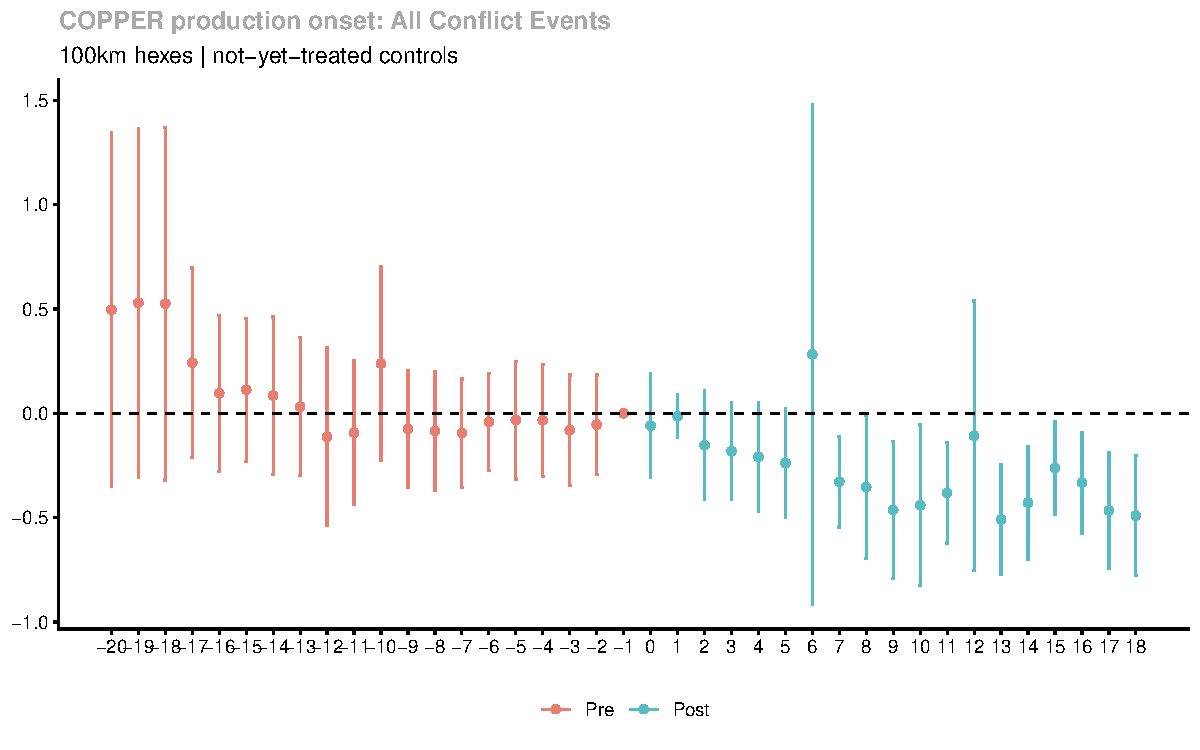
\includegraphics[width=0.48\textwidth]{plots/prod_copper_events_count.pdf}
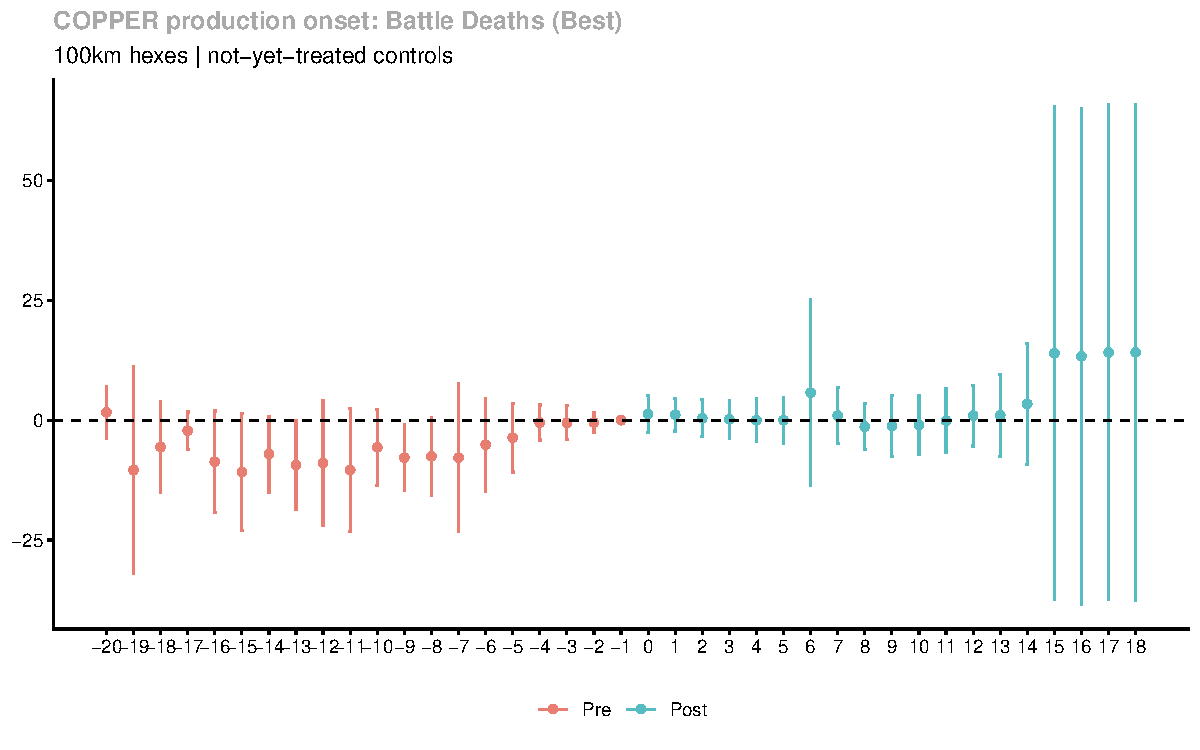
\includegraphics[width=0.48\textwidth]{plots/prod_copper_best_sum.pdf}
\caption{Copper production onset: conflict events (left) and battle deaths (right).}
\label{fig:prod_copper}
\end{figure}

\begin{figure}[H]
\centering
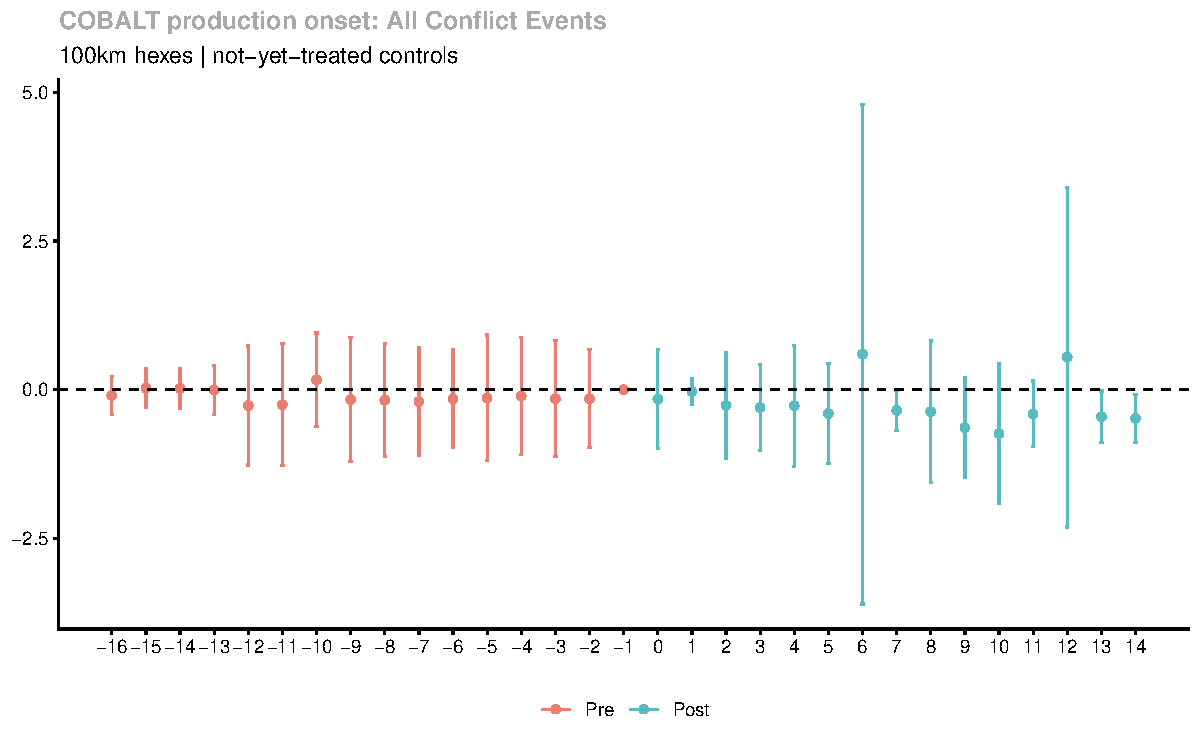
\includegraphics[width=0.48\textwidth]{plots/prod_cobalt_events_count.pdf}
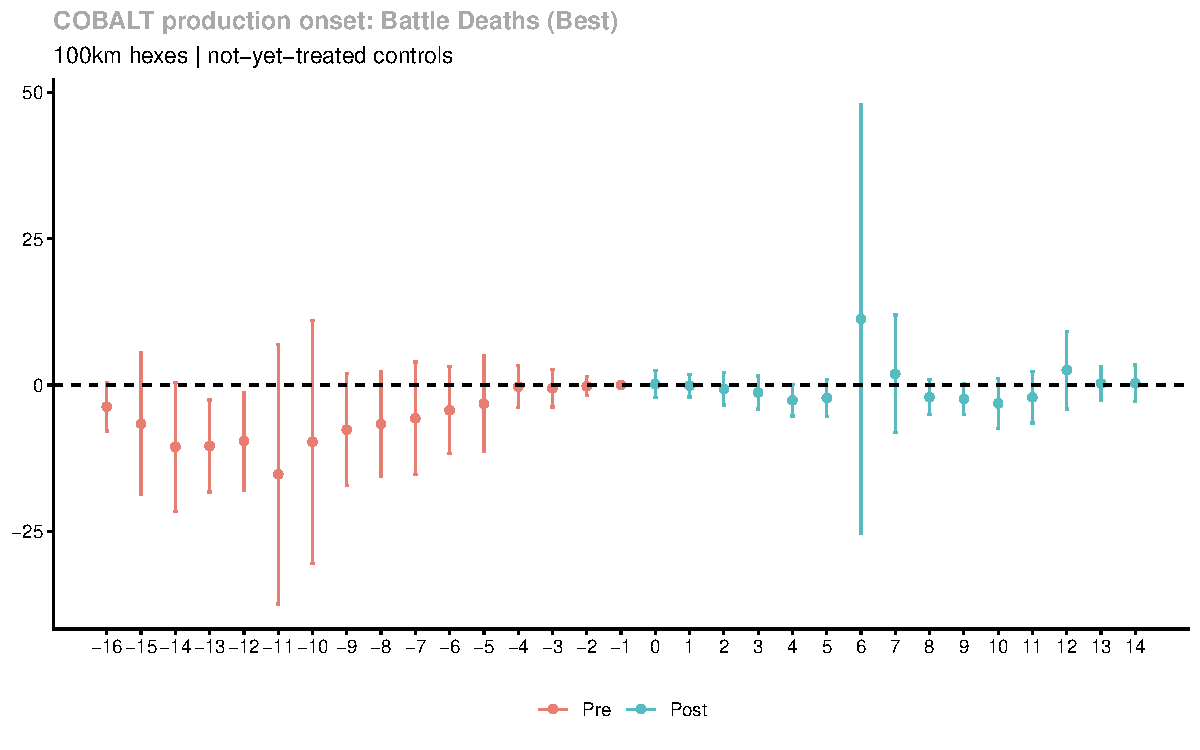
\includegraphics[width=0.48\textwidth]{plots/prod_cobalt_best_sum.pdf}
\caption{Cobalt production onset: conflict events (left) and battle deaths (right).}
\label{fig:prod_cobalt}
\end{figure}

\begin{figure}[H]
\centering
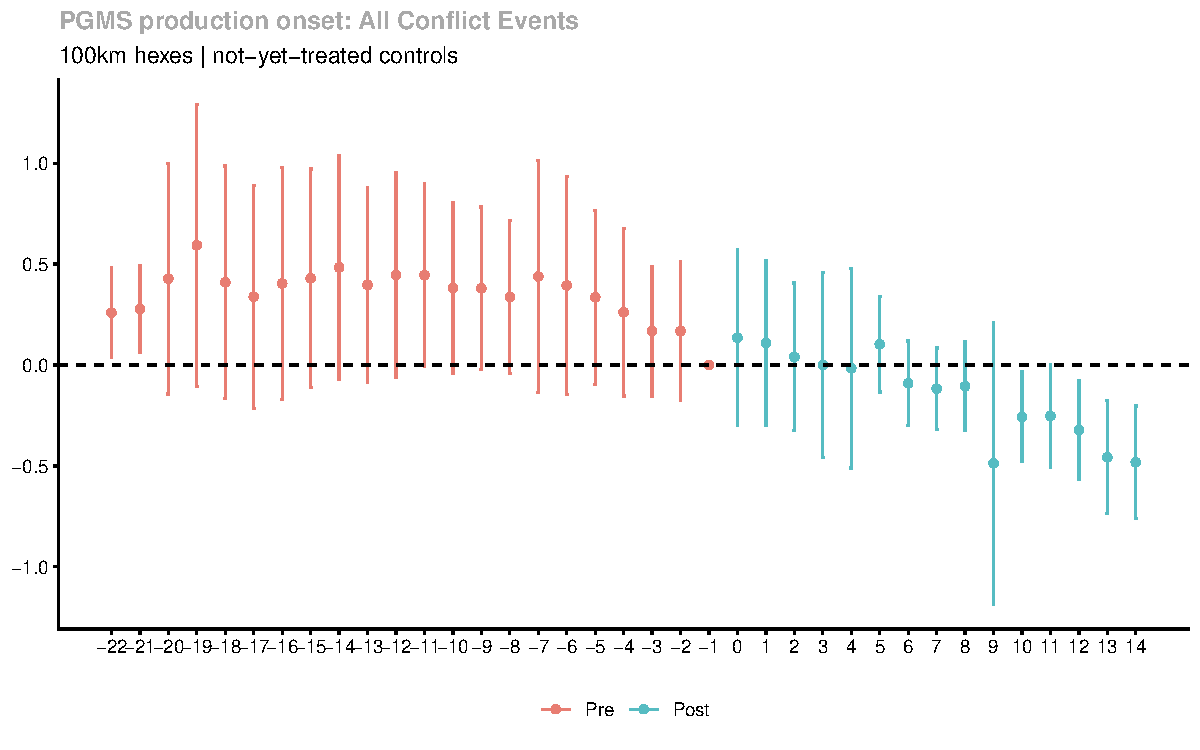
\includegraphics[width=0.48\textwidth]{plots/prod_pgms_events_count.pdf}
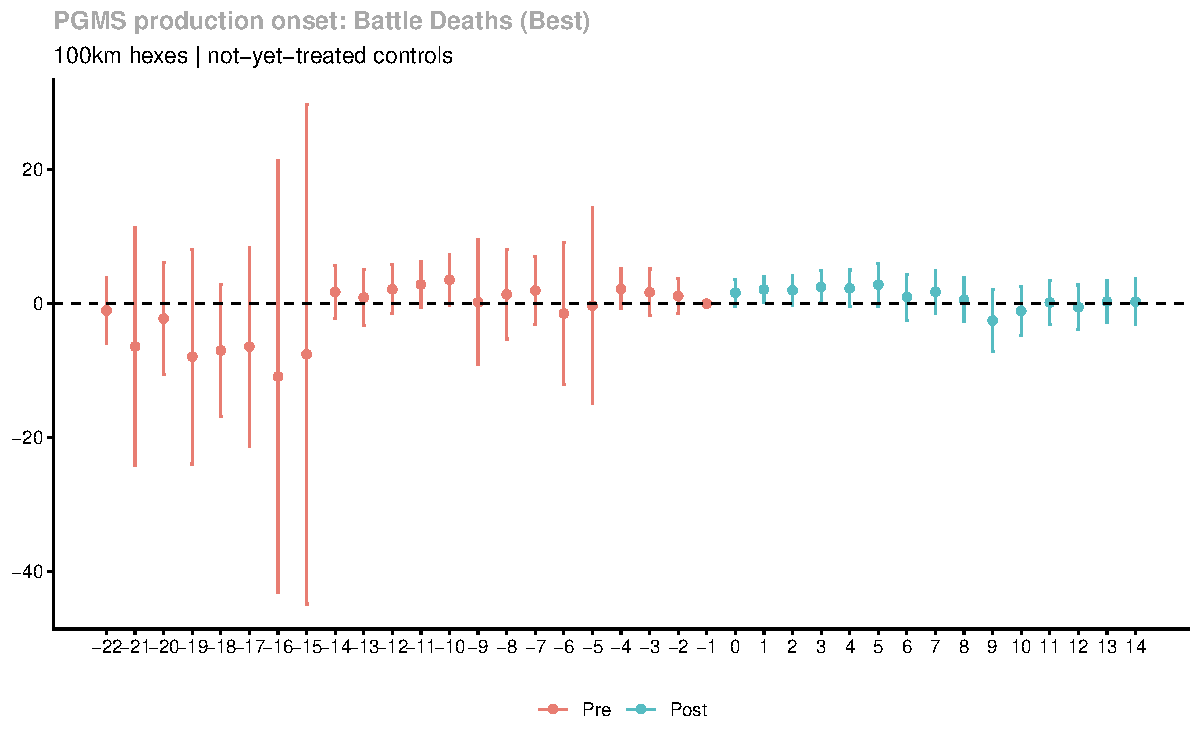
\includegraphics[width=0.48\textwidth]{plots/prod_pgms_best_sum.pdf}
\caption{PGMs production onset: conflict events (left) and battle deaths (right). Pre-trends are violated, so estimates are descriptive only.}
\label{fig:prod_pgms}
\end{figure}

\begin{figure}[H]
\centering
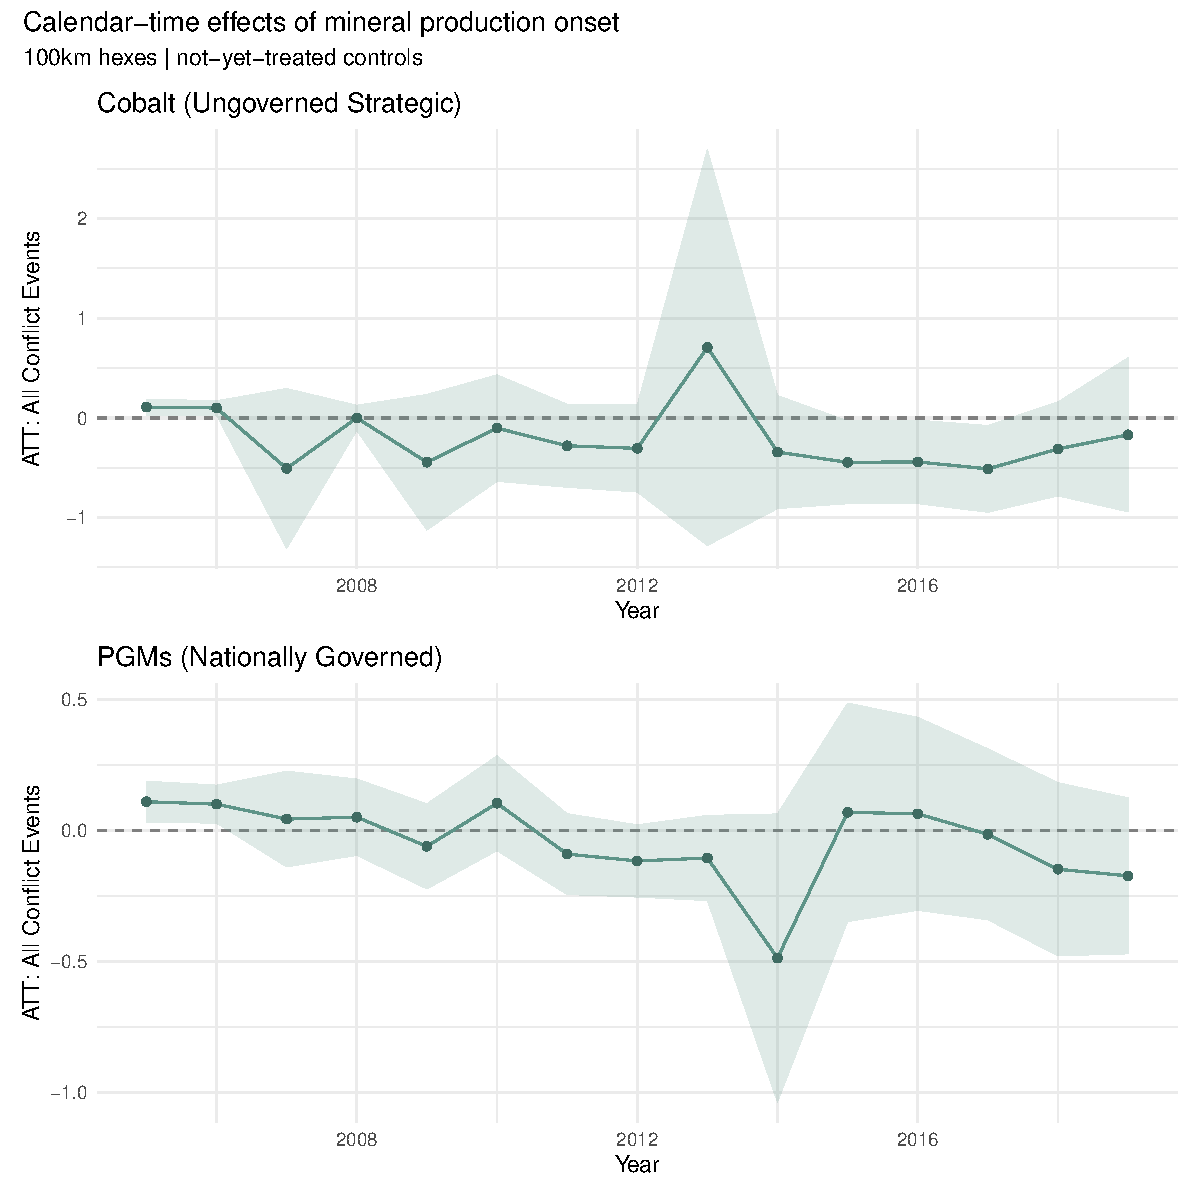
\includegraphics[width=0.7\textwidth]{plots/prod_calendar_comparison.pdf}
\caption{Calendar-time effects of production onset, cobalt and PGMs (conflict events).}
\label{fig:prod_calendar}
\end{figure}

\section{Full Results}
\setcounter{table}{0}
\setcounter{figure}{0}


\subsection{Pooled Effects}

\begin{longtable}{llrrrrr}
\caption{Pooled ATT Estimates Across Governance Tiers (100\,km Specification)} \label{tab:pooled_effects} \\
\toprule
\textbf{Mineral} & \textbf{Outcome} & \textbf{ATT} & \textbf{SE} & \textbf{p-value} & \textbf{\% $\Delta$} & \textbf{N Treated} \\
\midrule
\endfirsthead
\bottomrule
\endlastfoot
Tantalum & All Conflict Events & $-0.0297$ & 0.1336 & 0.824 & $-7$\% & 4 \\
Tantalum & Battle Deaths (Best) & $7.2868$ & 6.5459 & 0.266 & $+109$\% & 4 \\
\midrule
Chromium & All Conflict Events & $-0.0439$ & 0.1024 & 0.668 & $-10$\% & 6 \\
Chromium & Battle Deaths (Best) & $1.6831$ & 2.1450 & 0.433 & $+25$\% & 6 \\
\midrule
PGMs & All Conflict Events & $-0.0337$ & 0.1847 & 0.855 & $-8$\% & 4 \\
PGMs & Battle Deaths (Best) & $8.9393$ & 9.9037 & 0.367 & $+134$\% & 4 \\
\end{longtable}


\subsection{Tantalum (3T Governed)}

\begin{longtable}{lrrr}
\caption{Tantalum: effect of discovery on conflict events, by years since discovery (100\,km)} \label{tab:tantalum_all_conflict_events} \\
\toprule
\textbf{Years since discovery} & \textbf{ATT} & \textbf{SE} & \textbf{95\% CI} \\
\midrule \endfirsthead
\toprule
\textbf{Years since discovery} & \textbf{ATT} & \textbf{SE} & \textbf{95\% CI} \\
\midrule \endhead
\bottomrule \endlastfoot
-23 & 0.3325$^{***}$ & 0.0893 & [0.158, 0.507] \\
-22 & 0.0521 & 0.6621 & [-1.246, 1.350] \\
-21 & 0.7189 & 1.0956 & [-1.428, 2.866] \\
-20 & 0.2190 & 0.5421 & [-0.844, 1.282] \\
-19 & 2.3742 & 2.6987 & [-2.915, 7.664] \\
-18 & 1.3301 & 0.9415 & [-0.515, 3.175] \\
-17 & 2.4067 & 2.3386 & [-2.177, 6.990] \\
-16 & 4.4269 & 3.8867 & [-3.191, 12.045] \\
-15 & 1.1930 & 1.5890 & [-1.921, 4.307] \\
-14 & 0.0022 & 0.3142 & [-0.614, 0.618] \\
-13 & -0.0196 & 0.3086 & [-0.624, 0.585] \\
-12 & 0.4822 & 0.4979 & [-0.494, 1.458] \\
-11 & -0.0552 & 0.2843 & [-0.612, 0.502] \\
-10 & 0.1261 & 0.4157 & [-0.689, 0.941] \\
-9 & -0.0744 & 0.2745 & [-0.612, 0.464] \\
-8 & -0.1552 & 0.2382 & [-0.622, 0.312] \\
-7 & -0.1102 & 0.2255 & [-0.552, 0.332] \\
-6 & 0.0303 & 0.2368 & [-0.434, 0.494] \\
-5 & -0.1226 & 0.2548 & [-0.622, 0.377] \\
-4 & -0.1466 & 0.2490 & [-0.635, 0.341] \\
-3 & -0.2762 & 0.2103 & [-0.688, 0.136] \\
-2 & -0.1629 & 0.1706 & [-0.497, 0.171] \\
-1 & 0.0000 & NA & [NA, NA] \\
0 & -0.2037 & 0.2344 & [-0.663, 0.256] \\
1 & -0.2934 & 0.3625 & [-1.004, 0.417] \\
2 & 0.1641 & 0.7825 & [-1.370, 1.698] \\
3 & -0.0030 & 0.3891 & [-0.766, 0.760] \\
4 & 0.0282 & 0.3617 & [-0.681, 0.737] \\
5 & -0.3985 & 0.5304 & [-1.438, 0.641] \\
6 & -0.1874$^{**}$ & 0.0734 & [-0.331, -0.043] \\
7 & -0.2418$^{*}$ & 0.1278 & [-0.492, 0.009] \\
8 & -0.2004 & 0.1467 & [-0.488, 0.087] \\
9 & -0.1696 & 0.1039 & [-0.373, 0.034] \\
10 & -0.2244$^{**}$ & 0.0905 & [-0.402, -0.047] \\
11 & -0.2918$^{***}$ & 0.1059 & [-0.499, -0.084] \\
12 & -0.0612 & 0.3408 & [-0.729, 0.607] \\
13 & -0.3420$^{**}$ & 0.1438 & [-0.624, -0.060] \\
14 & -0.2700$^{***}$ & 0.0855 & [-0.438, -0.102] \\
15 & 0.0457 & 0.3606 & [-0.661, 0.752] \\
16 & -0.4856$^{***}$ & 0.1276 & [-0.736, -0.236] \\
17 & 0.1068 & 0.2836 & [-0.449, 0.663] \\
18 & -0.3121$^{***}$ & 0.0829 & [-0.475, -0.150] \\
19 & -0.3848$^{***}$ & 0.0881 & [-0.557, -0.212] \\
20 & -0.5200$^{***}$ & 0.1078 & [-0.731, -0.309] \\
\end{longtable}


\begin{longtable}{lrrr}
\caption{Tantalum: effect of discovery on battle deaths, by years since discovery (100\,km)} \label{tab:tantalum_battle_deaths_best_} \\
\toprule
\textbf{Years since discovery} & \textbf{ATT} & \textbf{SE} & \textbf{95\% CI} \\
\midrule \endfirsthead
\toprule
\textbf{Years since discovery} & \textbf{ATT} & \textbf{SE} & \textbf{95\% CI} \\
\midrule \endhead
\bottomrule \endlastfoot
-23 & 0.7512 & 1.1537 & [-1.510, 3.012] \\
-22 & -25.4611 & 26.4917 & [-77.385, 26.463] \\
-21 & -22.2990 & 23.4564 & [-68.274, 23.676] \\
-20 & -20.1197 & 21.3947 & [-62.053, 21.814] \\
-19 & 304.0054 & 397.8383 & [-475.758, 1083.768] \\
-18 & 9.2687 & 26.1145 & [-41.916, 60.453] \\
-17 & 50.0900 & 87.8609 & [-122.117, 222.297] \\
-16 & 229.7758 & 266.3361 & [-292.243, 751.795] \\
-15 & 11.8352 & 35.7937 & [-58.320, 81.991] \\
-14 & -15.1279 & 11.1931 & [-37.066, 6.811] \\
-13 & -12.4723 & 11.1483 & [-34.323, 9.378] \\
-12 & -1.3796 & 11.7724 & [-24.453, 21.694] \\
-11 & -8.6150 & 10.5171 & [-29.229, 11.999] \\
-10 & -8.1703 & 10.7125 & [-29.167, 12.826] \\
-9 & -7.7080 & 10.6187 & [-28.521, 13.105] \\
-8 & -7.7394 & 10.7559 & [-28.821, 13.342] \\
-7 & -6.9469 & 10.1803 & [-26.900, 13.006] \\
-6 & -5.8803 & 9.7852 & [-25.059, 13.299] \\
-5 & -6.7861 & 9.8814 & [-26.154, 12.582] \\
-4 & -5.9215 & 8.6850 & [-22.944, 11.101] \\
-3 & -7.2295 & 9.0917 & [-25.049, 10.590] \\
-2 & -7.5018 & 8.5557 & [-24.271, 9.267] \\
-1 & 0.0000 & NA & [NA, NA] \\
0 & -6.2647 & 9.5923 & [-25.066, 12.536] \\
1 & 0.9150 & 7.0757 & [-12.953, 14.783] \\
2 & -0.7539 & 1.5763 & [-3.843, 2.336] \\
3 & 0.2583 & 1.8466 & [-3.361, 3.878] \\
4 & 8.0153 & 9.7520 & [-11.099, 27.129] \\
5 & 0.5980 & 2.5453 & [-4.391, 5.587] \\
6 & 2.6122 & 3.5360 & [-4.318, 9.543] \\
7 & 2.8021 & 4.0575 & [-5.151, 10.755] \\
8 & 3.4680 & 4.5731 & [-5.495, 12.431] \\
9 & 4.0689 & 5.0566 & [-5.842, 13.980] \\
10 & 3.8437 & 4.3350 & [-4.653, 12.340] \\
11 & 3.5311 & 4.3634 & [-5.021, 12.083] \\
12 & 5.0495 & 6.0786 & [-6.865, 16.964] \\
13 & 5.8739 & 6.5695 & [-7.002, 18.750] \\
14 & 7.0595 & 6.8924 & [-6.450, 20.569] \\
15 & 7.2169 & 6.7239 & [-5.962, 20.396] \\
16 & 5.8650 & 6.5908 & [-7.053, 18.783] \\
17 & 11.3977 & 10.1335 & [-8.464, 31.259] \\
18 & 6.9405$^{**}$ & 3.3949 & [0.287, 13.595] \\
19 & 6.2323$^{*}$ & 3.6253 & [-0.873, 13.338] \\
20 & 7.0317$^{**}$ & 3.3628 & [0.441, 13.623] \\
\end{longtable}


\begin{longtable}{lrrr}
\caption{Tantalum: calendar-time effect of discovery on battle deaths (100\,km)} \label{tab:cal_tantalum} \\
\toprule
\textbf{Year} & \textbf{ATT} & \textbf{SE} & \textbf{95\% CI} \\
\midrule \endfirsthead
\toprule
\textbf{Year} & \textbf{ATT} & \textbf{SE} & \textbf{95\% CI} \\
\midrule \endhead
\bottomrule \endlastfoot
1998 & 2.2108 & 3.3442 & [-4.344, 8.766] \\
1999 & -9.0256 & 12.1333 & [-32.807, 14.756] \\
2000 & -7.1572 & 19.9753 & [-46.309, 31.995] \\
2001 & 10.5871 & 9.9241 & [-8.864, 30.038] \\
2002 & 5.4608 & 7.0097 & [-8.278, 19.200] \\
2003 & 6.4021 & 6.7042 & [-6.738, 19.542] \\
2004 & 6.7757 & 6.8206 & [-6.593, 20.144] \\
2005 & 10.1140 & 6.6056 & [-2.833, 23.061] \\
2006 & 6.9216 & 5.3330 & [-3.531, 17.374] \\
2007 & 5.9958 & 4.5579 & [-2.938, 14.929] \\
2008 & 48.7319 & 50.1041 & [-49.472, 146.936] \\
2009 & 4.0330 & 4.4850 & [-4.758, 12.824] \\
2010 & 5.7071 & 4.3703 & [-2.859, 14.273] \\
2011 & 2.8696 & 3.9167 & [-4.807, 10.546] \\
2012 & 3.2581 & 3.1968 & [-3.008, 9.524] \\
2013 & 1.9201 & 2.4767 & [-2.934, 6.774] \\
2014 & -3.2810 & 2.2916 & [-7.773, 1.211] \\
2015 & -1.6381 & 2.0259 & [-5.609, 2.333] \\
2016 & 0.7121 & 1.8078 & [-2.831, 4.255] \\
2017 & -3.3853 & 10.8098 & [-24.572, 17.802] \\
2018 & -5.8997 & 9.6264 & [-24.767, 12.968] \\
\end{longtable}


\begin{table}[H]
\centering
\caption{Tantalum Effects Across Spatial Scales. Cells report the number of significant post-treatment periods (at $p<0.05$) with direction of effect in parentheses. ``---'' indicates no significant effects.}
\label{tab:tantalum_robustness}
\begin{tabular}{lcccccc}
\toprule
Scale & All Events & Battle Deaths & State-Based & Non-State & One-Sided & Pre-Trends \\
\midrule
300km & 7 (Neg)   & ---           & 4 (Neg)     & ---       & ---       & 0--4       \\
250km & ---       & ---           & 3 (Neg)     & 20 (Neg)  & ---       & 3--4       \\
200km & ---       & ---           & ---         & ---       & ---       & ---        \\
150km & ---       & ---           & 8 (Neg)     & ---       & 9 (Neg)   & 2--5       \\
100km & ---       & 9 (Neg)       & ---         & ---       & 7 (Neg)   & 2--3       \\
050km & ---       & ---           & ---         & 5 (Neg)   & ---       & 0          \\
025km & ---       & ---           & ---         & ---       & ---       & ---        \\
\bottomrule
\end{tabular}
\end{table}

\subsection{Tin (3T Governed)}

Tin provides additional evidence for the effectiveness of 3T governance frameworks. Like tantalum, tin shows strong pacification effects with no increase in battle deaths, supporting H1.

\begin{table}[H]
\centering
\caption{Tin Effects Across Spatial Scales. Cells report the number of significant post-treatment periods (at $p<0.05$) with direction of effect in parentheses. ``---'' indicates no significant effects. Tin shows particularly strong effects at coarser scales (200--250km), consistent with regional supply chain mechanisms.}
\label{tab:tin_robustness}
\begin{tabular}{lcccccc}
\toprule
Scale & All Events & Battle Deaths & State-Based & Non-State & One-Sided & Pre-Trends \\
\midrule
300km & ---       & ---           & 7 (Neg)     & 4 (Neg)   & ---       & 3--5       \\
250km & ---       & ---           & ---         & 20 (Neg)  & ---       & 3          \\
200km & ---       & ---           & ---         & 20 (Neg)  & ---       & 5          \\
150km & ---       & ---           & ---         & 5 (Neg)   & ---       & 4          \\
100km & ---       & ---           & ---         & ---       & ---       & ---        \\
050km & ---       & ---           & ---         & ---       & ---       & ---        \\
025km & ---       & ---           & ---         & ---       & ---       & ---        \\
\bottomrule
\end{tabular}
\end{table}

\subsection{Chromium (Governance Gap)}

\begin{longtable}{lrrr}
\caption{Chromium: effect of discovery on conflict events, by years since discovery (100\,km)} \label{tab:chromium_all_conflict_events} \\
\toprule
\textbf{Years since discovery} & \textbf{ATT} & \textbf{SE} & \textbf{95\% CI} \\
\midrule \endfirsthead
\toprule
\textbf{Years since discovery} & \textbf{ATT} & \textbf{SE} & \textbf{95\% CI} \\
\midrule \endhead
\bottomrule \endlastfoot
-23 & 0.3304$^{***}$ & 0.0908 & [0.152, 0.508] \\
-22 & 0.6994$^{**}$ & 0.3262 & [0.060, 1.339] \\
-21 & 0.3584$^{***}$ & 0.0897 & [0.182, 0.534] \\
-20 & 0.3324$^{**}$ & 0.1649 & [0.009, 0.656] \\
-19 & 0.3828$^{**}$ & 0.1524 & [0.084, 0.682] \\
-18 & 0.4084$^{***}$ & 0.1564 & [0.102, 0.715] \\
-17 & 0.4156$^{***}$ & 0.1345 & [0.152, 0.679] \\
-16 & 0.3573$^{***}$ & 0.1231 & [0.116, 0.599] \\
-15 & 0.4085$^{***}$ & 0.1453 & [0.124, 0.693] \\
-14 & 0.4337$^{***}$ & 0.1220 & [0.195, 0.673] \\
-13 & 0.4444$^{***}$ & 0.1252 & [0.199, 0.690] \\
-12 & 0.3020$^{**}$ & 0.1252 & [0.057, 0.547] \\
-11 & 0.3576$^{***}$ & 0.1288 & [0.105, 0.610] \\
-10 & 1.1253 & 1.1120 & [-1.054, 3.305] \\
-9 & 0.2813$^{*}$ & 0.1539 & [-0.020, 0.583] \\
-8 & 0.2925 & 0.1897 & [-0.079, 0.664] \\
-7 & 0.2413$^{**}$ & 0.1207 & [0.005, 0.478] \\
-6 & 0.1414$^{*}$ & 0.0835 & [-0.022, 0.305] \\
-5 & 0.1518 & 0.1017 & [-0.048, 0.351] \\
-4 & 0.0199 & 0.0666 & [-0.111, 0.150] \\
-3 & 0.0736 & 0.0690 & [-0.062, 0.209] \\
-2 & 0.1077 & 0.0720 & [-0.034, 0.249] \\
-1 & 0.0000 & NA & [NA, NA] \\
0 & 0.0148 & 0.0677 & [-0.118, 0.148] \\
1 & 0.0677 & 0.0776 & [-0.084, 0.220] \\
2 & 0.0424 & 0.0873 & [-0.129, 0.213] \\
3 & 0.0187 & 0.0805 & [-0.139, 0.177] \\
4 & -0.0421 & 0.0713 & [-0.182, 0.098] \\
5 & 0.1077 & 0.2476 & [-0.378, 0.593] \\
6 & -0.0925 & 0.0825 & [-0.254, 0.069] \\
7 & -0.1966 & 0.1600 & [-0.510, 0.117] \\
8 & -0.2232$^{*}$ & 0.1247 & [-0.468, 0.021] \\
9 & -0.2502$^{**}$ & 0.1096 & [-0.465, -0.035] \\
10 & -0.2512$^{**}$ & 0.1016 & [-0.450, -0.052] \\
11 & -0.3431$^{**}$ & 0.1463 & [-0.630, -0.056] \\
12 & -0.2777$^{**}$ & 0.1270 & [-0.527, -0.029] \\
13 & -0.2333$^{*}$ & 0.1388 & [-0.505, 0.039] \\
14 & -0.1511 & 0.1304 & [-0.407, 0.105] \\
15 & -0.4092$^{**}$ & 0.1607 & [-0.724, -0.094] \\
16 & -0.1571$^{*}$ & 0.0954 & [-0.344, 0.030] \\
17 & -0.1530 & 0.0931 & [-0.336, 0.030] \\
18 & -0.2235$^{**}$ & 0.0991 & [-0.418, -0.029] \\
19 & -0.3570$^{***}$ & 0.1250 & [-0.602, -0.112] \\
\end{longtable}


\begin{longtable}{lrrr}
\caption{Chromium: effect of discovery on battle deaths, by years since discovery (100\,km)} \label{tab:chromium_battle_deaths_best_} \\
\toprule
\textbf{Years since discovery} & \textbf{ATT} & \textbf{SE} & \textbf{95\% CI} \\
\midrule \endfirsthead
\toprule
\textbf{Years since discovery} & \textbf{ATT} & \textbf{SE} & \textbf{95\% CI} \\
\midrule \endhead
\bottomrule \endlastfoot
-23 & -0.3488 & 1.7449 & [-3.769, 3.071] \\
-22 & -10.3532 & 8.5393 & [-27.090, 6.384] \\
-21 & -7.5862$^{**}$ & 3.6262 & [-14.694, -0.479] \\
-20 & -2.0307 & 2.0104 & [-5.971, 1.910] \\
-19 & -13.2593$^{*}$ & 7.6229 & [-28.200, 1.682] \\
-18 & -10.2149 & 11.9874 & [-33.710, 13.280] \\
-17 & -0.5440 & 1.4126 & [-3.313, 2.225] \\
-16 & -5.7505 & 5.0437 & [-15.636, 4.135] \\
-15 & -4.4283 & 7.7733 & [-19.664, 10.807] \\
-14 & 1.4178 & 1.1333 & [-0.803, 3.639] \\
-13 & 2.7984$^{**}$ & 1.1466 & [0.551, 5.046] \\
-12 & 0.9731 & 1.3016 & [-1.578, 3.524] \\
-11 & -2.0349 & 3.4191 & [-8.736, 4.667] \\
-10 & 0.6530 & 2.5578 & [-4.360, 5.666] \\
-9 & -2.6899 & 2.5856 & [-7.758, 2.378] \\
-8 & -2.9414 & 3.5750 & [-9.948, 4.066] \\
-7 & -5.4319 & 5.6503 & [-16.506, 5.643] \\
-6 & -3.0347 & 3.5893 & [-10.070, 4.000] \\
-5 & -1.4509 & 2.3502 & [-6.057, 3.156] \\
-4 & -1.8006 & 1.7884 & [-5.306, 1.705] \\
-3 & -2.1761 & 2.1218 & [-6.335, 1.983] \\
-2 & 0.3988 & 0.7645 & [-1.100, 1.897] \\
-1 & 0.0000 & NA & [NA, NA] \\
0 & -0.0819 & 1.5459 & [-3.112, 2.948] \\
1 & -0.0221 & 2.3853 & [-4.697, 4.653] \\
2 & 1.6383 & 1.1047 & [-0.527, 3.804] \\
3 & 1.7416$^{*}$ & 0.8985 & [-0.019, 3.503] \\
4 & 1.0559 & 1.1899 & [-1.276, 3.388] \\
5 & 1.2267 & 1.2955 & [-1.313, 3.766] \\
6 & 1.0085 & 1.8484 & [-2.614, 4.632] \\
7 & 0.0731 & 2.2656 & [-4.368, 4.514] \\
8 & -0.4054 & 2.1568 & [-4.633, 3.822] \\
9 & -0.2501 & 1.9351 & [-4.043, 3.543] \\
10 & -0.4271 & 1.7041 & [-3.767, 2.913] \\
11 & -0.2963 & 2.0255 & [-4.266, 3.674] \\
12 & 0.6536 & 1.9182 & [-3.106, 4.413] \\
13 & 2.8455 & 2.2067 & [-1.480, 7.171] \\
14 & 3.1973 & 2.0993 & [-0.917, 7.312] \\
15 & 2.0459 & 1.4608 & [-0.817, 4.909] \\
16 & 3.8969$^{**}$ & 1.8214 & [0.327, 7.467] \\
17 & 5.1804$^{***}$ & 1.8700 & [1.515, 8.846] \\
18 & 4.4944$^{**}$ & 1.7610 & [1.043, 7.946] \\
19 & 5.3162$^{***}$ & 1.7789 & [1.829, 8.803] \\
\end{longtable}


\begin{longtable}{lrrr}
\caption{Chromium: calendar-time effect of discovery on battle deaths (100\,km)} \label{tab:cal_chromium} \\
\toprule
\textbf{Year} & \textbf{ATT} & \textbf{SE} & \textbf{95\% CI} \\
\midrule \endfirsthead
\toprule
\textbf{Year} & \textbf{ATT} & \textbf{SE} & \textbf{95\% CI} \\
\midrule \endhead
\bottomrule \endlastfoot
1999 & -10.7115 & 10.7179 & [-31.719, 10.295] \\
2000 & -8.8155 & 19.6910 & [-47.410, 29.779] \\
2001 & 5.2416$^{***}$ & 1.5538 & [2.196, 8.287] \\
2002 & 3.7050$^{*}$ & 1.9238 & [-0.066, 7.476] \\
2003 & 2.7922 & 1.8725 & [-0.878, 6.462] \\
2004 & 3.1642 & 2.0185 & [-0.792, 7.120] \\
2005 & 5.4350$^{***}$ & 1.6915 & [2.120, 8.750] \\
2006 & 3.4099$^{**}$ & 1.6536 & [0.169, 6.651] \\
2007 & 2.7301$^{*}$ & 1.4849 & [-0.180, 5.641] \\
2008 & 2.0122 & 1.3595 & [-0.652, 4.677] \\
2009 & 0.7792 & 1.5343 & [-2.228, 3.786] \\
2010 & 2.4474 & 1.5906 & [-0.670, 5.565] \\
2011 & 0.5683 & 1.5004 & [-2.373, 3.509] \\
2012 & 1.3591 & 1.4633 & [-1.509, 4.227] \\
2013 & 0.2025 & 1.4910 & [-2.720, 3.125] \\
2014 & -2.9219 & 1.9474 & [-6.739, 0.895] \\
2015 & -0.7752 & 1.2777 & [-3.280, 1.729] \\
2016 & 0.5083 & 1.2644 & [-1.970, 2.987] \\
2017 & -0.1777 & 1.2939 & [-2.714, 2.358] \\
2018 & 0.6925 & 0.8644 & [-1.002, 2.387] \\
\end{longtable}


% TODO: Chromium scale sensitivity table (populate from multi-scale analysis)

\subsection{Platinum Group Metals (Nationally Governed)}

\begin{longtable}{rrrrrr}
\caption{Dynamic ATT Estimates for PGMs, Nationally Governed (All Conflict Events)} \label{tab:pgms_all_conflict_events} \\
\toprule
\textbf{Event Time} & \textbf{ATT} & \textbf{SE} & \textbf{CI Lower} & \textbf{CI Upper} & \textbf{p-value} \\
\midrule
\endfirsthead
\multicolumn{6}{c}{\textit{Continued from previous page}} \\
\toprule
\textbf{Event Time} & \textbf{ATT} & \textbf{SE} & \textbf{CI Lower} & \textbf{CI Upper} & \textbf{p-value} \\
\midrule
\endhead
\midrule \multicolumn{6}{r}{\textit{Continued on next page}} \\
\endfoot
\bottomrule
\endlastfoot
-15 & 0.3667$^{*}$ & 0.0794 & 0.2111 & 0.5224 & $<$0.001 \\
-14 & 0.2293$^{*}$ & 0.0891 & 0.0547 & 0.4040 & 0.010 \\
-13 & 0.2824$^{*}$ & 0.0830 & 0.1197 & 0.4452 & $<$0.001 \\
-12 & 0.0811 & 0.1371 & -0.1876 & 0.3499 & 0.554 \\
-11 & 0.0674 & 0.1477 & -0.2221 & 0.3570 & 0.648 \\
-10 & 0.0739 & 0.1379 & -0.1963 & 0.3441 & 0.592 \\
-9 & 1.3428 & 1.0968 & -0.8070 & 3.4926 & 0.221 \\
-8 & 1.6532 & 1.6044 & -1.4914 & 4.7977 & 0.303 \\
-7 & 0.9860 & 0.9328 & -0.8424 & 2.8143 & 0.291 \\
-6 & 0.7567 & 0.7681 & -0.7487 & 2.2621 & 0.325 \\
-5 & 0.0209 & 0.5667 & -1.0898 & 1.1316 & 0.971 \\
-4 & -0.2483 & 0.2486 & -0.7355 & 0.2389 & 0.318 \\
-3 & -0.2401 & 0.2387 & -0.7080 & 0.2277 & 0.314 \\
-2 & -0.3482 & 0.2615 & -0.8607 & 0.1643 & 0.183 \\
-1 & 0.0000NA & NA & NA & NA & NA \\
0 & 0.9973 & 0.8388 & -0.6468 & 2.6415 & 0.234 \\
1 & -0.2579 & 0.2282 & -0.7052 & 0.1895 & 0.259 \\
2 & -0.3522 & 0.2342 & -0.8113 & 0.1069 & 0.133 \\
3 & -0.3676 & 0.2813 & -0.9191 & 0.1838 & 0.191 \\
4 & -0.3864 & 0.2872 & -0.9494 & 0.1766 & 0.179 \\
5 & -0.4234 & 0.2177 & -0.8500 & 0.0033 & 0.052 \\
6 & 0.5688 & 0.7768 & -0.9538 & 2.0914 & 0.464 \\
7 & 3.4269 & 3.7806 & -3.9831 & 10.8369 & 0.365 \\
8 & -0.6220$^{*}$ & 0.1743 & -0.9636 & -0.2803 & $<$0.001 \\
9 & 0.4196 & 0.7730 & -1.0955 & 1.9348 & 0.587 \\
10 & -0.5480$^{*}$ & 0.1623 & -0.8661 & -0.2299 & $<$0.001 \\
11 & -0.6805$^{*}$ & 0.1851 & -1.0434 & -0.3176 & $<$0.001 \\
12 & -0.3220 & 0.2152 & -0.7438 & 0.0999 & 0.135 \\
13 & -1.0676$^{*}$ & 0.0869 & -1.2378 & -0.8973 & $<$0.001 \\
14 & -1.4496$^{*}$ & 0.3263 & -2.0891 & -0.8102 & $<$0.001 \\
15 & -0.2181$^{*}$ & 0.0870 & -0.3885 & -0.0477 & 0.012 \\
16 & -1.2143$^{*}$ & 0.0915 & -1.3937 & -1.0349 & $<$0.001 \\
17 & -1.2846$^{*}$ & 0.0946 & -1.4700 & -1.0992 & $<$0.001 \\
18 & -1.4179$^{*}$ & 0.1150 & -1.6433 & -1.1925 & $<$0.001 \\
\end{longtable}


\begin{longtable}{lrrr}
\caption{PGMs: effect of discovery on battle deaths, by years since discovery (100\,km)} \label{tab:pgms_battle_deaths_best_} \\
\toprule
\textbf{Years since discovery} & \textbf{ATT} & \textbf{SE} & \textbf{95\% CI} \\
\midrule \endfirsthead
\toprule
\textbf{Years since discovery} & \textbf{ATT} & \textbf{SE} & \textbf{95\% CI} \\
\midrule \endhead
\bottomrule \endlastfoot
-21 & 0.2468 & 1.7139 & [-3.112, 3.606] \\
-20 & -11.7551 & 7.9869 & [-27.409, 3.899] \\
-19 & -6.9838$^{*}$ & 3.6481 & [-14.134, 0.167] \\
-18 & -3.8912$^{*}$ & 2.0312 & [-7.872, 0.090] \\
-17 & -14.5918 & 11.3654 & [-36.868, 7.684] \\
-16 & -8.1995 & 9.9915 & [-27.783, 11.384] \\
-15 & -7.1767 & 7.4584 & [-21.795, 7.442] \\
-14 & -5.5623 & 4.3911 & [-14.169, 3.044] \\
-13 & -3.5470 & 3.2373 & [-9.892, 2.798] \\
-12 & -6.9850 & 6.3319 & [-19.396, 5.426] \\
-11 & -7.2254 & 4.8437 & [-16.719, 2.268] \\
-10 & -8.3948$^{*}$ & 4.7651 & [-17.734, 0.945] \\
-9 & -3.6848 & 3.8695 & [-11.269, 3.899] \\
-8 & -3.3447 & 3.1951 & [-9.607, 2.918] \\
-7 & -8.8092 & 8.9384 & [-26.329, 8.710] \\
-6 & 1.6135 & 6.7456 & [-11.608, 14.835] \\
-5 & 1.2187 & 4.6424 & [-7.880, 10.318] \\
-4 & -0.3713 & 4.7706 & [-9.722, 8.979] \\
-3 & 1.6082 & 4.0031 & [-6.238, 9.454] \\
-2 & -0.8736 & 2.6300 & [-6.028, 4.281] \\
-1 & 0.0000 & NA & [NA, NA] \\
0 & 3.3217 & 2.2688 & [-1.125, 7.769] \\
1 & 2.2094 & 3.3588 & [-4.374, 8.793] \\
2 & 1.9998 & 2.6334 & [-3.162, 7.161] \\
3 & 3.7232 & 4.5389 & [-5.173, 12.620] \\
4 & 4.4285 & 4.5964 & [-4.581, 13.437] \\
5 & 4.7022 & 4.7064 & [-4.522, 13.927] \\
6 & 6.8318 & 5.9097 & [-4.751, 18.415] \\
7 & 7.4668 & 6.9281 & [-6.112, 21.046] \\
8 & 4.3999 & 5.7089 & [-6.790, 15.589] \\
9 & 31.9008 & 35.8085 & [-38.284, 102.086] \\
10 & 5.3843 & 5.5573 & [-5.508, 16.277] \\
11 & 4.9134 & 5.6336 & [-6.128, 15.955] \\
12 & 7.1484 & 6.7827 & [-6.146, 20.443] \\
13 & 11.5447 & 10.6982 & [-9.424, 32.513] \\
14 & 11.2395 & 10.7054 & [-9.743, 32.222] \\
15 & 12.7533 & 10.9873 & [-8.782, 34.289] \\
16 & 10.9114 & 10.5044 & [-9.677, 31.500] \\
17 & 11.4286 & 10.6881 & [-9.520, 32.377] \\
18 & 11.1373$^{*}$ & 6.1134 & [-0.845, 23.119] \\
19 & 7.5800$^{**}$ & 3.6064 & [0.511, 14.649] \\
20 & 8.4011$^{**}$ & 3.4061 & [1.725, 15.077] \\
\end{longtable}


\begin{longtable}{lrrr}
\caption{PGMs: calendar-time effect of discovery on battle deaths (100\,km)} \label{tab:cal_pgms} \\
\toprule
\textbf{Year} & \textbf{ATT} & \textbf{SE} & \textbf{95\% CI} \\
\midrule \endfirsthead
\toprule
\textbf{Year} & \textbf{ATT} & \textbf{SE} & \textbf{95\% CI} \\
\midrule \endhead
\bottomrule \endlastfoot
1998 & 3.0926 & 3.4599 & [-3.689, 9.874] \\
1999 & -7.6079 & 12.5443 & [-32.195, 16.979] \\
2000 & 2.5911 & 13.7675 & [-24.393, 29.575] \\
2001 & 12.1081 & 10.4948 & [-8.462, 32.678] \\
2002 & 10.5657 & 10.6127 & [-10.235, 31.366] \\
2003 & 11.5037 & 10.6475 & [-9.365, 32.373] \\
2004 & 11.8755 & 11.0711 & [-9.824, 33.575] \\
2005 & 15.1983 & 10.7300 & [-5.833, 36.229] \\
2006 & 11.4573 & 7.5505 & [-3.342, 26.256] \\
2007 & 11.0053 & 7.4749 & [-3.645, 25.656] \\
2008 & 6.7828 & 5.3912 & [-3.784, 17.350] \\
2009 & 32.2613 & 35.7397 & [-37.789, 102.311] \\
2010 & 7.2176 & 5.6925 & [-3.940, 18.375] \\
2011 & 4.3090 & 4.7923 & [-5.084, 13.702] \\
2012 & 5.2423 & 5.1331 & [-4.819, 15.303] \\
2013 & 3.9435 & 4.5961 & [-5.065, 12.952] \\
2014 & 0.8216 & 4.9657 & [-8.911, 10.554] \\
2015 & 2.6661 & 5.2376 & [-7.600, 12.932] \\
2016 & 3.2395 & 4.0553 & [-4.709, 11.188] \\
2017 & 2.5540 & 4.2713 & [-5.818, 10.926] \\
2018 & 3.3751 & 4.2716 & [-4.997, 11.747] \\
\end{longtable}


\begin{table}[H]
\centering
\caption{PGMs Effects Across Spatial Scales. Cells report the number of significant post-treatment periods (at $p<0.05$) with direction of effect in parentheses. ``---'' indicates no significant effects.}
\label{tab:pgms_robustness}
\begin{tabular}{lcccccc}
\toprule
Scale & All Events & Battle Deaths & State-Based & Non-State & One-Sided & Pre-Trends \\
\midrule
300km & ---       & ---           & ---         & 8 (Neg)   & ---       & 1          \\
250km & 3 (Neg)   & ---           & 3 (Neg)     & 9 (Neg)   & ---       & 1--2       \\
200km & ---       & 7 (Neg)       & 7 (Neg)     & 10 (Neg)  & ---       & 0--4       \\
150km & ---       & ---           & ---         & 9 (Neg)   & ---       & 4          \\
100km & ---       & ---           & ---         & 11 (Neg)  & ---       & 5          \\
050km & ---       & ---           & 3 (Neg)     & 8 (Neg)   & ---       & 4          \\
025km & ---       & ---           & 3 (Neg)     & 8 (Neg)   & ---       & ---        \\
\bottomrule
\end{tabular}
\end{table}

\subsection{Mechanism Tables}

\begin{table}[H]
\centering
\footnotesize
\caption{Actor-level effects of Tantalum discovery (100\,km)}
\label{tab:mech_tantalum}
\begin{tabular}{lrrr}
\toprule
\textbf{Actor outcome} & \textbf{ATT} & \textbf{ATT ($e\geq10$)} & \textbf{Pre} \\
\midrule
Formal grp initiator (ev.) & -0.119$^{***}$ (0.030) & -0.132$^{***}$ (0.025) & 0 \\
Formal grp initiator (fat.) & -0.686$^{***}$ (0.179) & -0.801$^{***}$ (0.219) & 0 \\
Formal grp target (ev.) & -0.240$^{***}$ (0.085) & -0.256$^{***}$ (0.057) & 0 \\
Formal grp target (fat.) & -0.962$^{*}$ (0.567) & -0.706 (0.684) & 1 \\
State initiator (ev.) & -0.132 (0.105) & -0.251$^{***}$ (0.059) & 0 \\
State initiator (fat.) & 0.539 (0.881) & -0.359 (0.705) & 1 \\
Civilians target (ev.) & -0.014 (0.076) & -0.131$^{***}$ (0.026) & 0 \\
Civilians target (fat.) & 0.759 (0.799) & -0.528$^{**}$ (0.206) & 0 \\
\bottomrule
\end{tabular}
\begin{minipage}{0.9\textwidth}\vspace{4pt}\scriptsize \textit{Notes.} Dynamic Callaway--Sant'Anna aggregates, standard errors in parentheses. \textbf{Pre} counts pre-treatment coefficients outside the simultaneous confidence band in the ten years before discovery, which is the window the figures display. $^{*}p<0.10$, $^{**}p<0.05$, $^{***}p<0.01$.\end{minipage}
\end{table}


\begin{table}[H]
\centering
\footnotesize
\caption{Actor-level effects of PGMs discovery (100\,km)}
\label{tab:mech_pgms}
\begin{tabular}{lrrr}
\toprule
\textbf{Actor outcome} & \textbf{ATT} & \textbf{ATT ($e\geq10$)} & \textbf{Pre} \\
\midrule
Formal grp initiator (ev.) & -0.082$^{***}$ (0.019) & -0.131$^{***}$ (0.029) & 0 \\
Formal grp initiator (fat.) & -0.567$^{***}$ (0.185) & -0.610$^{***}$ (0.165) & 0 \\
Formal grp target (ev.) & -0.190$^{***}$ (0.046) & -0.289$^{***}$ (0.061) & 0 \\
Formal grp target (fat.) & -1.637$^{***}$ (0.324) & -2.267$^{***}$ (0.440) & 1 \\
State initiator (ev.) & -0.179$^{***}$ (0.052) & -0.271$^{***}$ (0.065) & 0 \\
State initiator (fat.) & -1.500$^{***}$ (0.311) & -1.951$^{***}$ (0.446) & 0 \\
Civilians target (ev.) & -0.073$^{***}$ (0.028) & -0.120$^{***}$ (0.031) & 0 \\
Civilians target (fat.) & -0.458$^{**}$ (0.179) & -0.388$^{**}$ (0.182) & 0 \\
\bottomrule
\end{tabular}
\begin{minipage}{0.9\textwidth}\vspace{4pt}\scriptsize \textit{Notes.} Dynamic Callaway--Sant'Anna aggregates, standard errors in parentheses. \textbf{Pre} counts pre-treatment coefficients outside the simultaneous confidence band in the ten years before discovery, which is the window the figures display. $^{*}p<0.10$, $^{**}p<0.05$, $^{***}p<0.01$.\end{minipage}
\end{table}


\begin{longtable}{lrrrrr}
\caption{Actor-Level Mechanism for Chromium (Ungoverned Strategic), 100\,km} \label{tab:mech_chromium} \\
\toprule
\textbf{Actor Outcome} & \textbf{Sig Post} & \textbf{Direction} & \textbf{Sig Pre} & \textbf{ATT} & \textbf{SE} \\
\midrule
\endfirsthead
\bottomrule
\endlastfoot
State initiator (events) & 0 & - & 4 & -0.0207 & 0.0674 \\
State initiator (fatal.) & 7 & Pos & 2 & 1.4669 & 1.8439 \\
Civilians target (fatal.) & 5 & Pos & 1 & 0.7944 & 0.6196 \\
\end{longtable}


\end{document}
